
	\item \textbf{L’interface de transfert
		:}La figure~\ref{transfert} montre l'historique des transactions de l'utilisateur  vers les bénéficiaires avec détails pour chaque transaction.
	
	\begin{figure}
		\centering
		\begin{subfigure}[b]{0.3\textwidth}
			\centering
			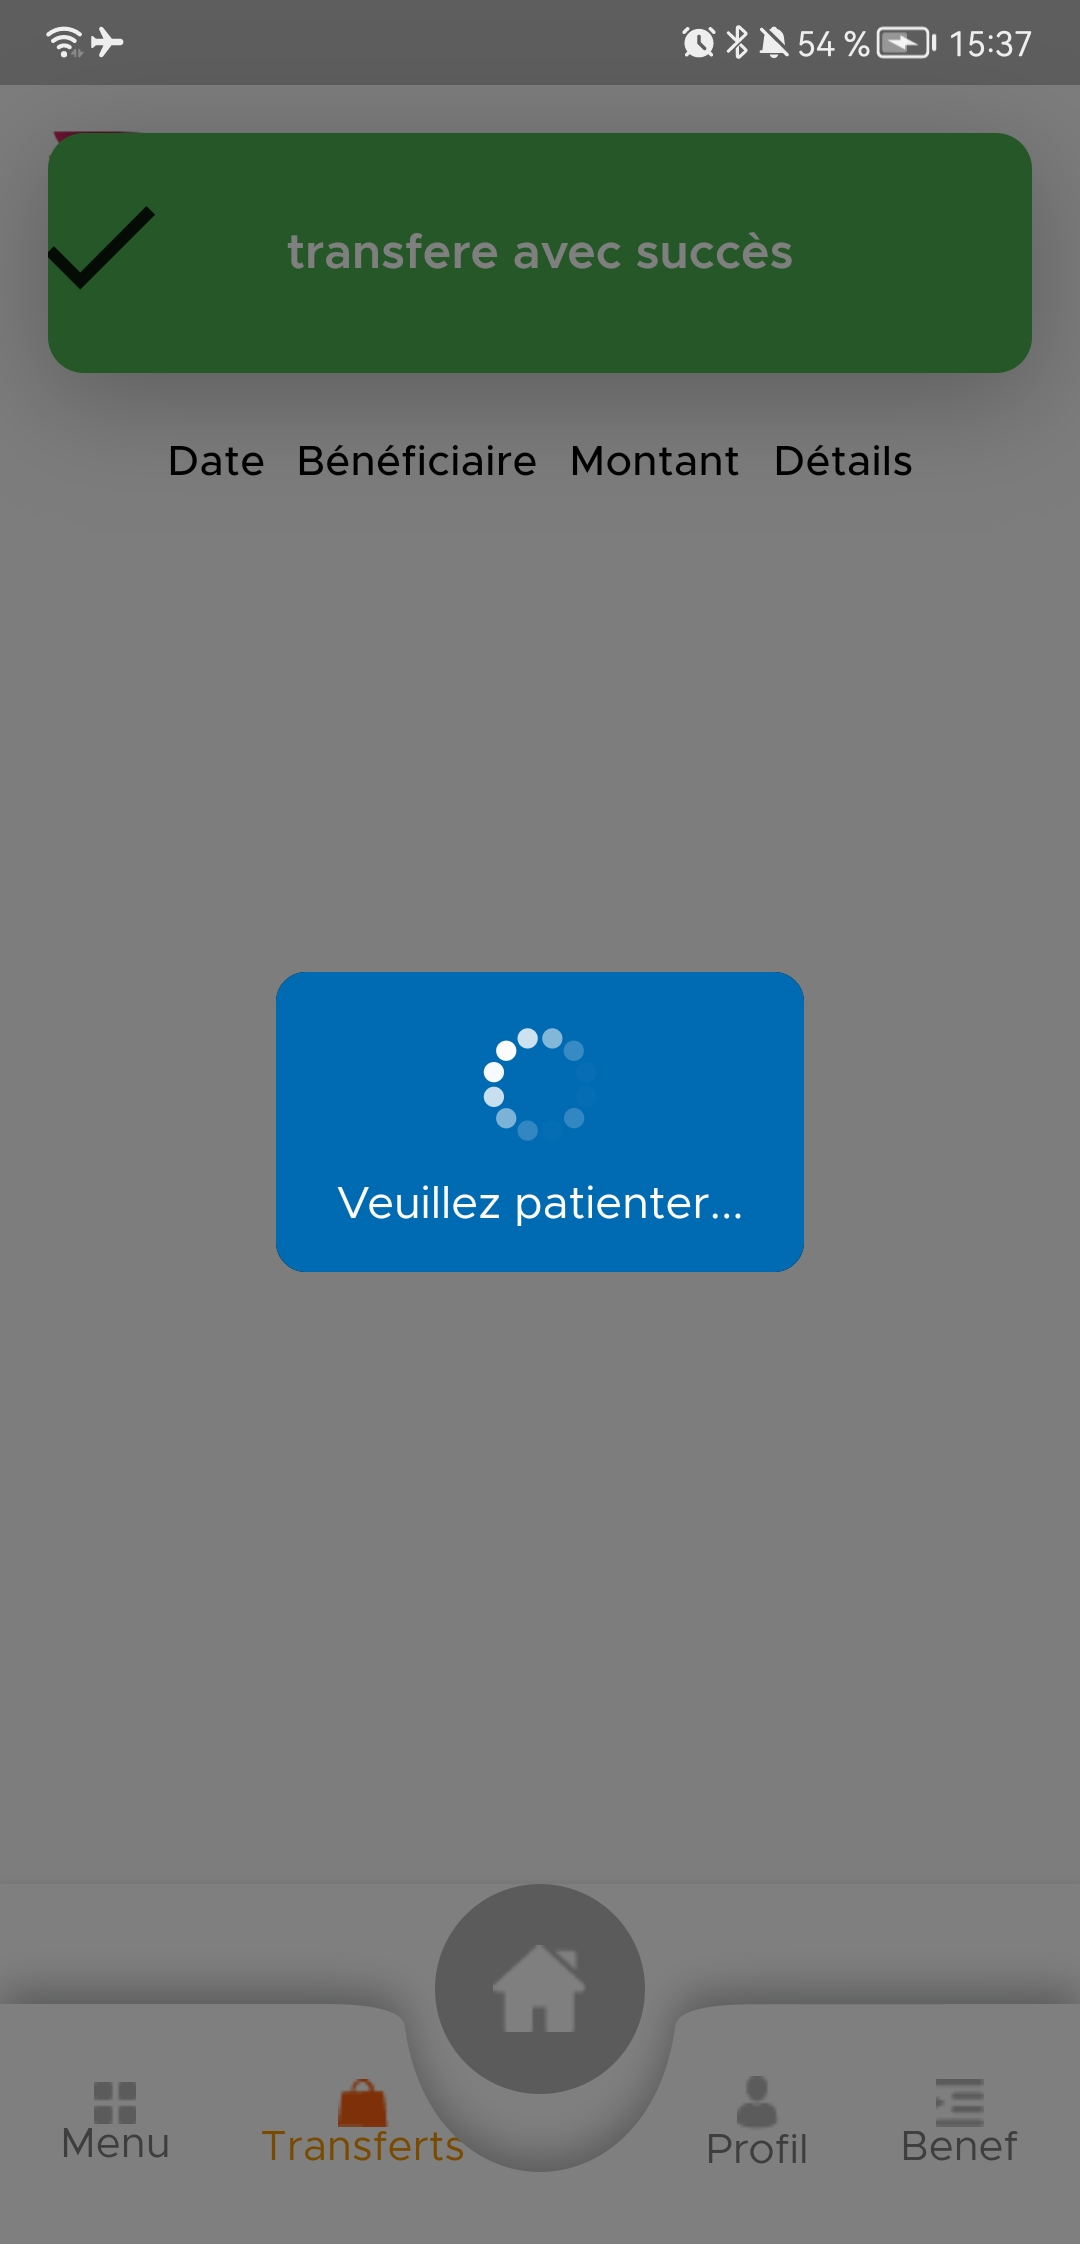
\includegraphics[width=\textwidth]{./Template LaTeX/Images/16.jpg}
			\caption{Transfere avec succés}
			\label{fig:y equals x}
		\end{subfigure}
		\hfill
		\begin{subfigure}[b]{0.3\textwidth}
			\centering
			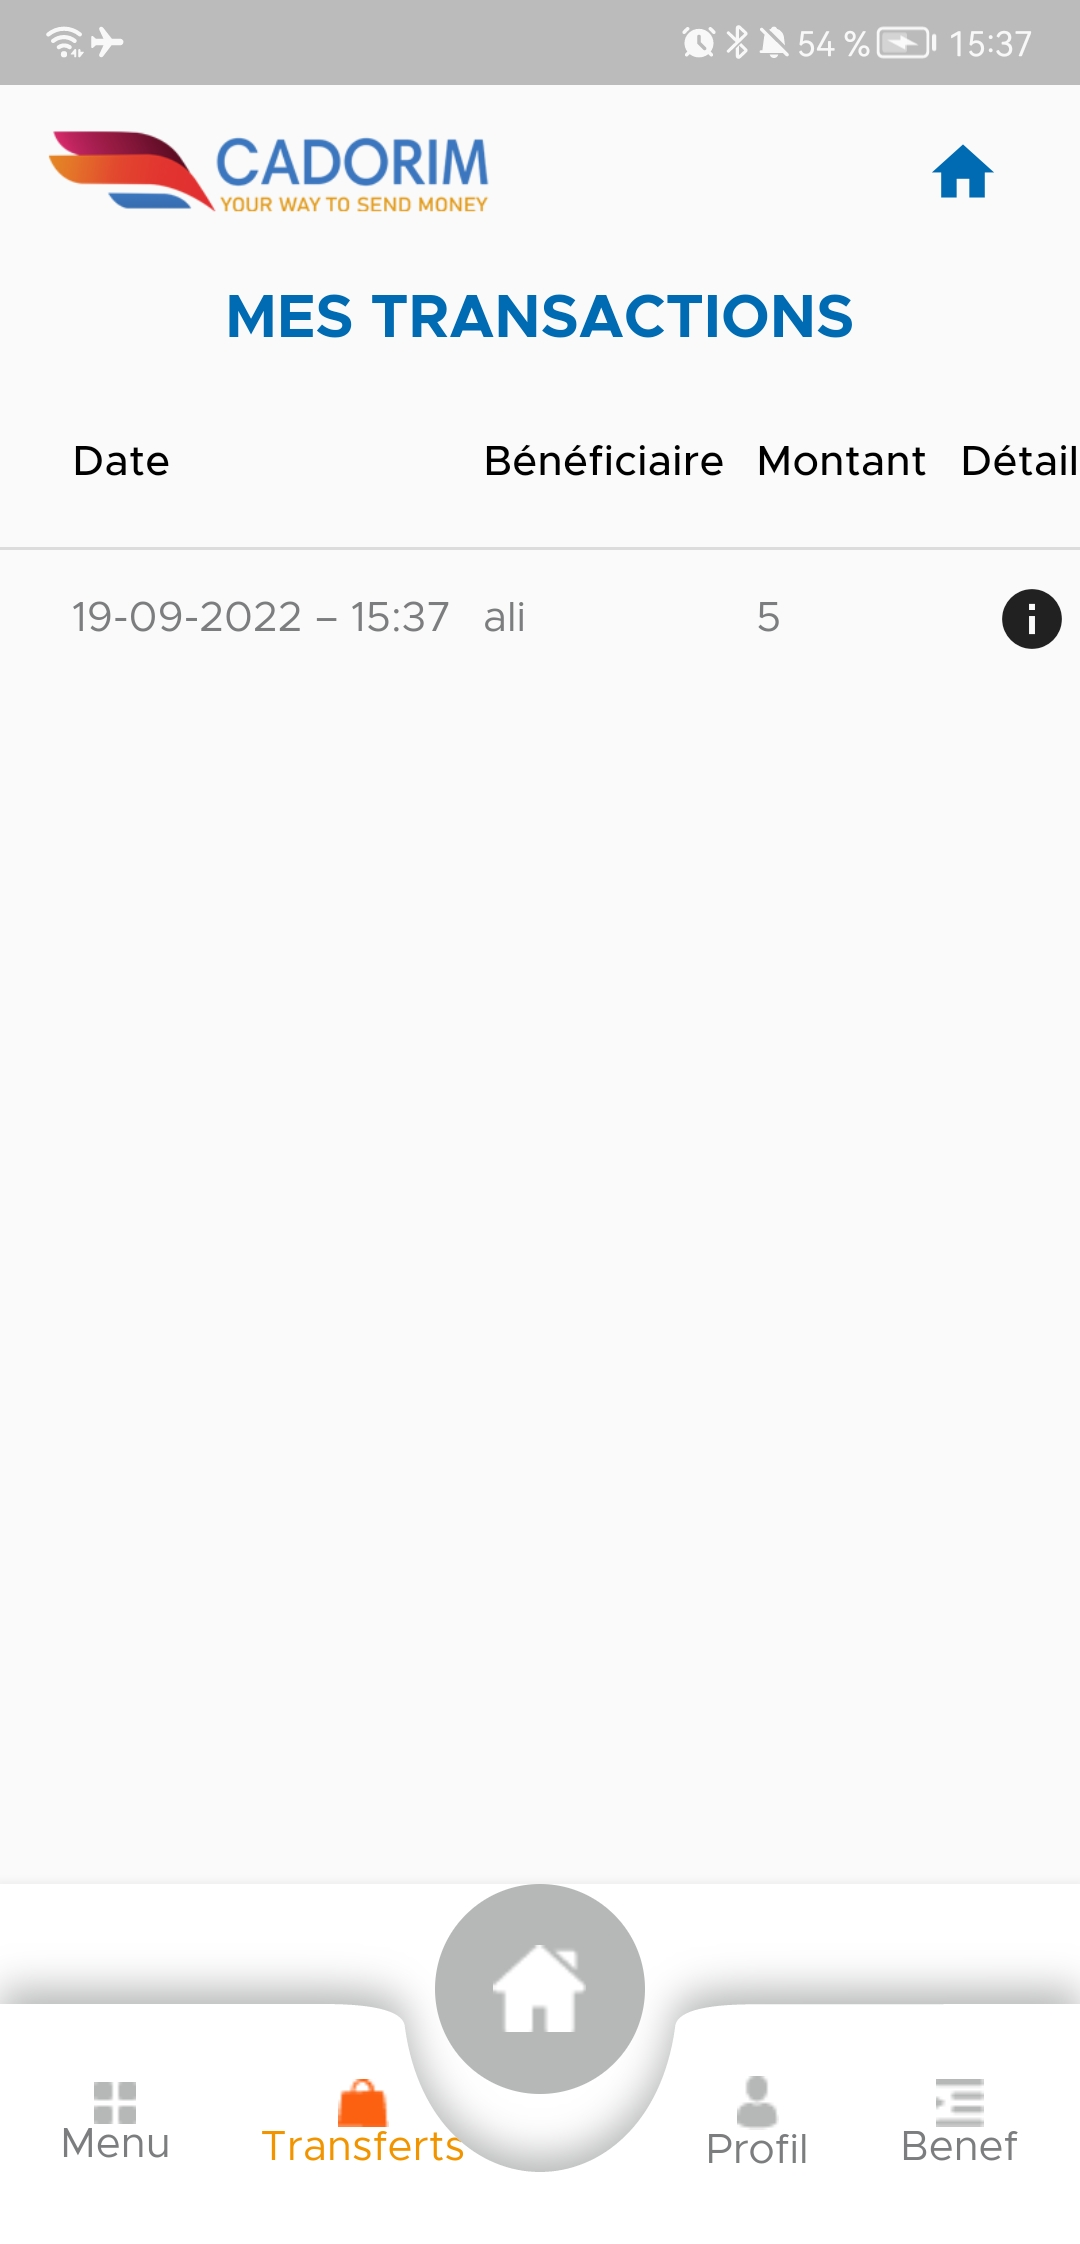
\includegraphics[width=\textwidth]{./Template LaTeX/Images/17.jpg}
			\caption{Historique transactions}
			\label{fig:three sin x}
		\end{subfigure}
		\hfill
		\begin{subfigure}[b]{0.3\textwidth}
			\centering
			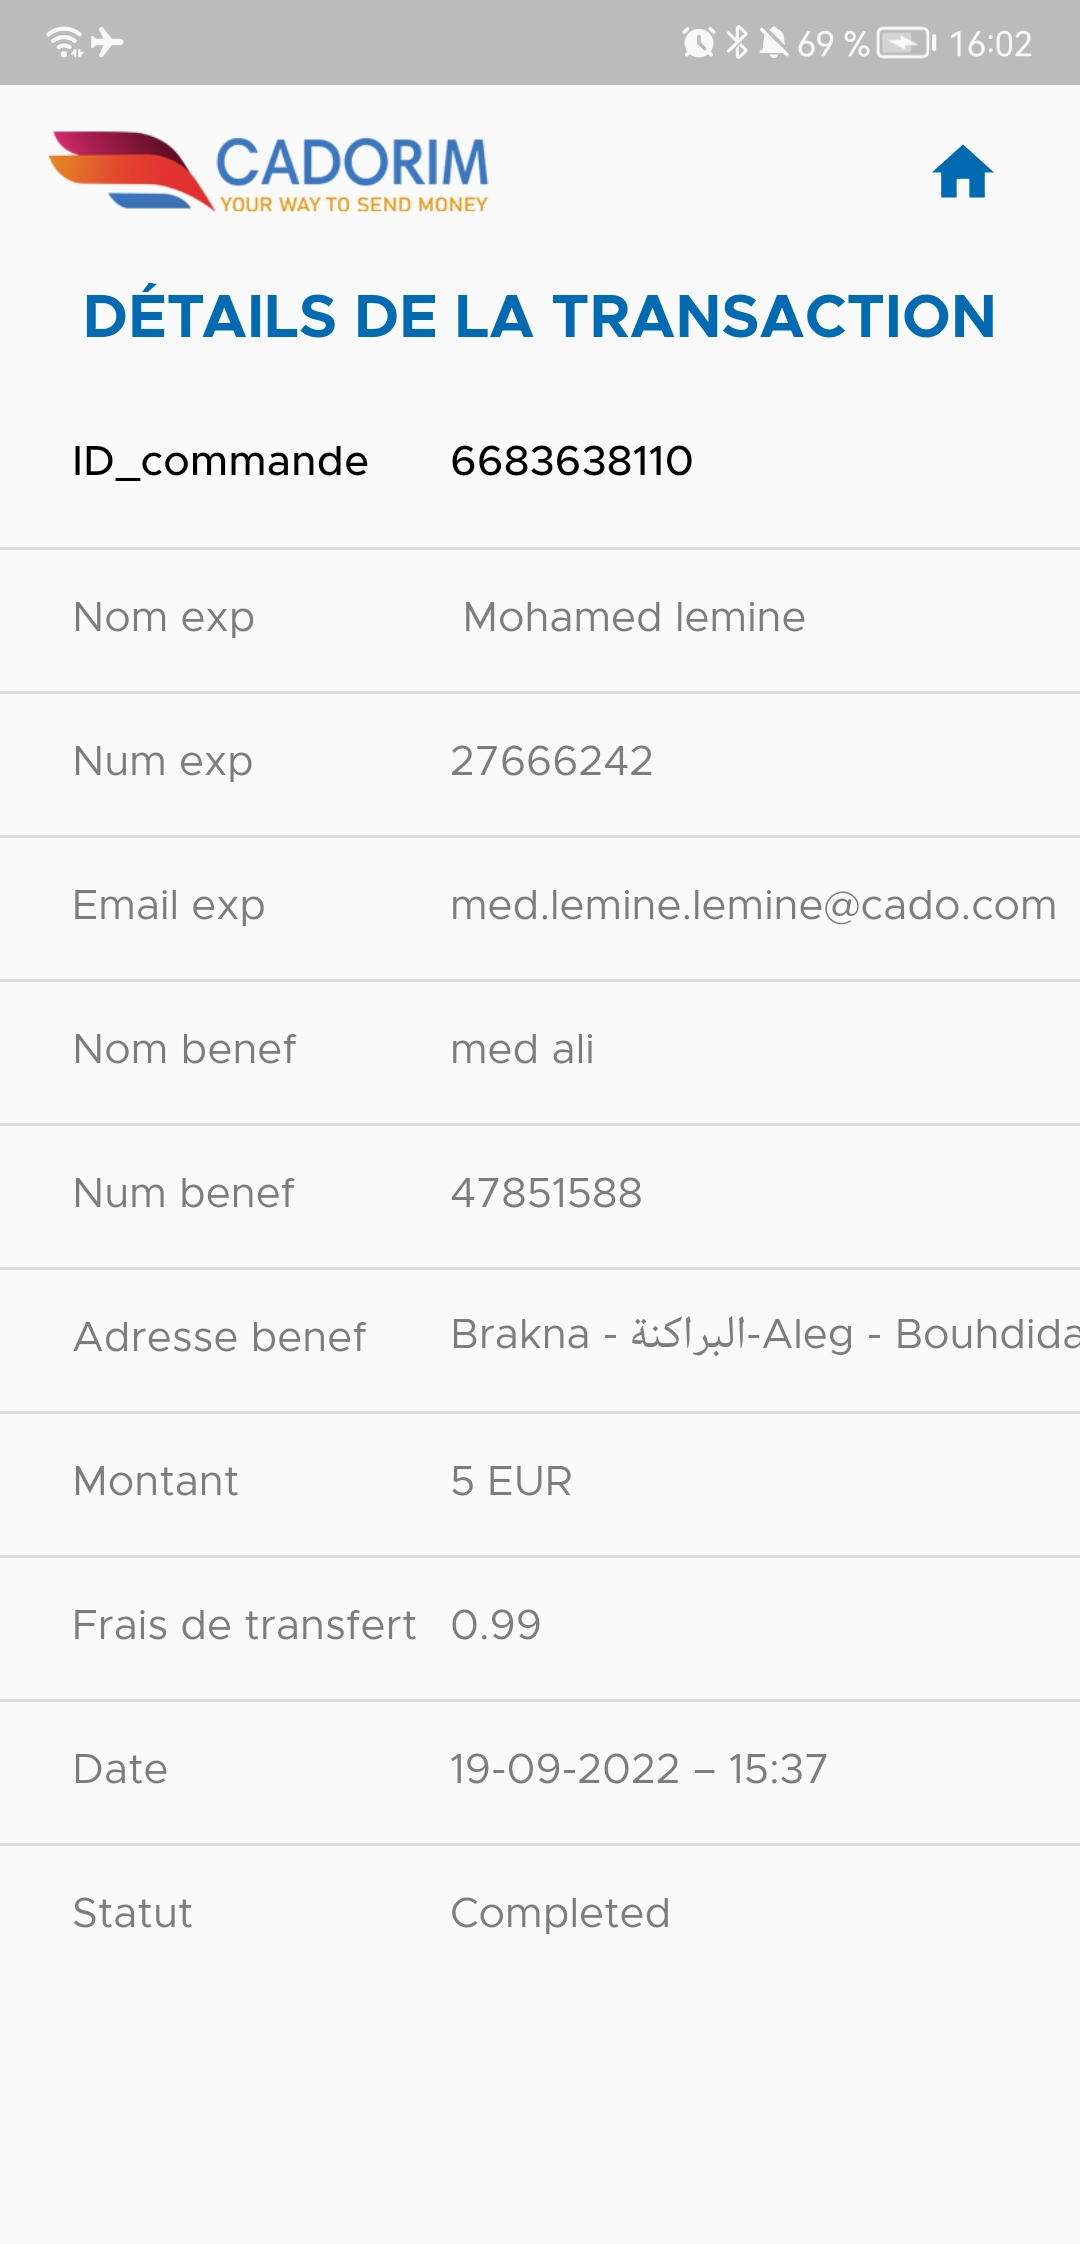
\includegraphics[width=\textwidth]{./Template LaTeX/Images/18.jpg}
			\caption{Détails de la transaction}
			\label{fig:five over x}
		\end{subfigure}
		\caption{Transferts}
		\label{transfert}
	\end{figure}
	
	\item \textbf{L’interface de discussion
		:} La figure suivante montre que le client peut envoyer un message (photo ou un texte) au service client et bien sur voir l'historique des messages.
	\begin{figure}%
		\centering
		{{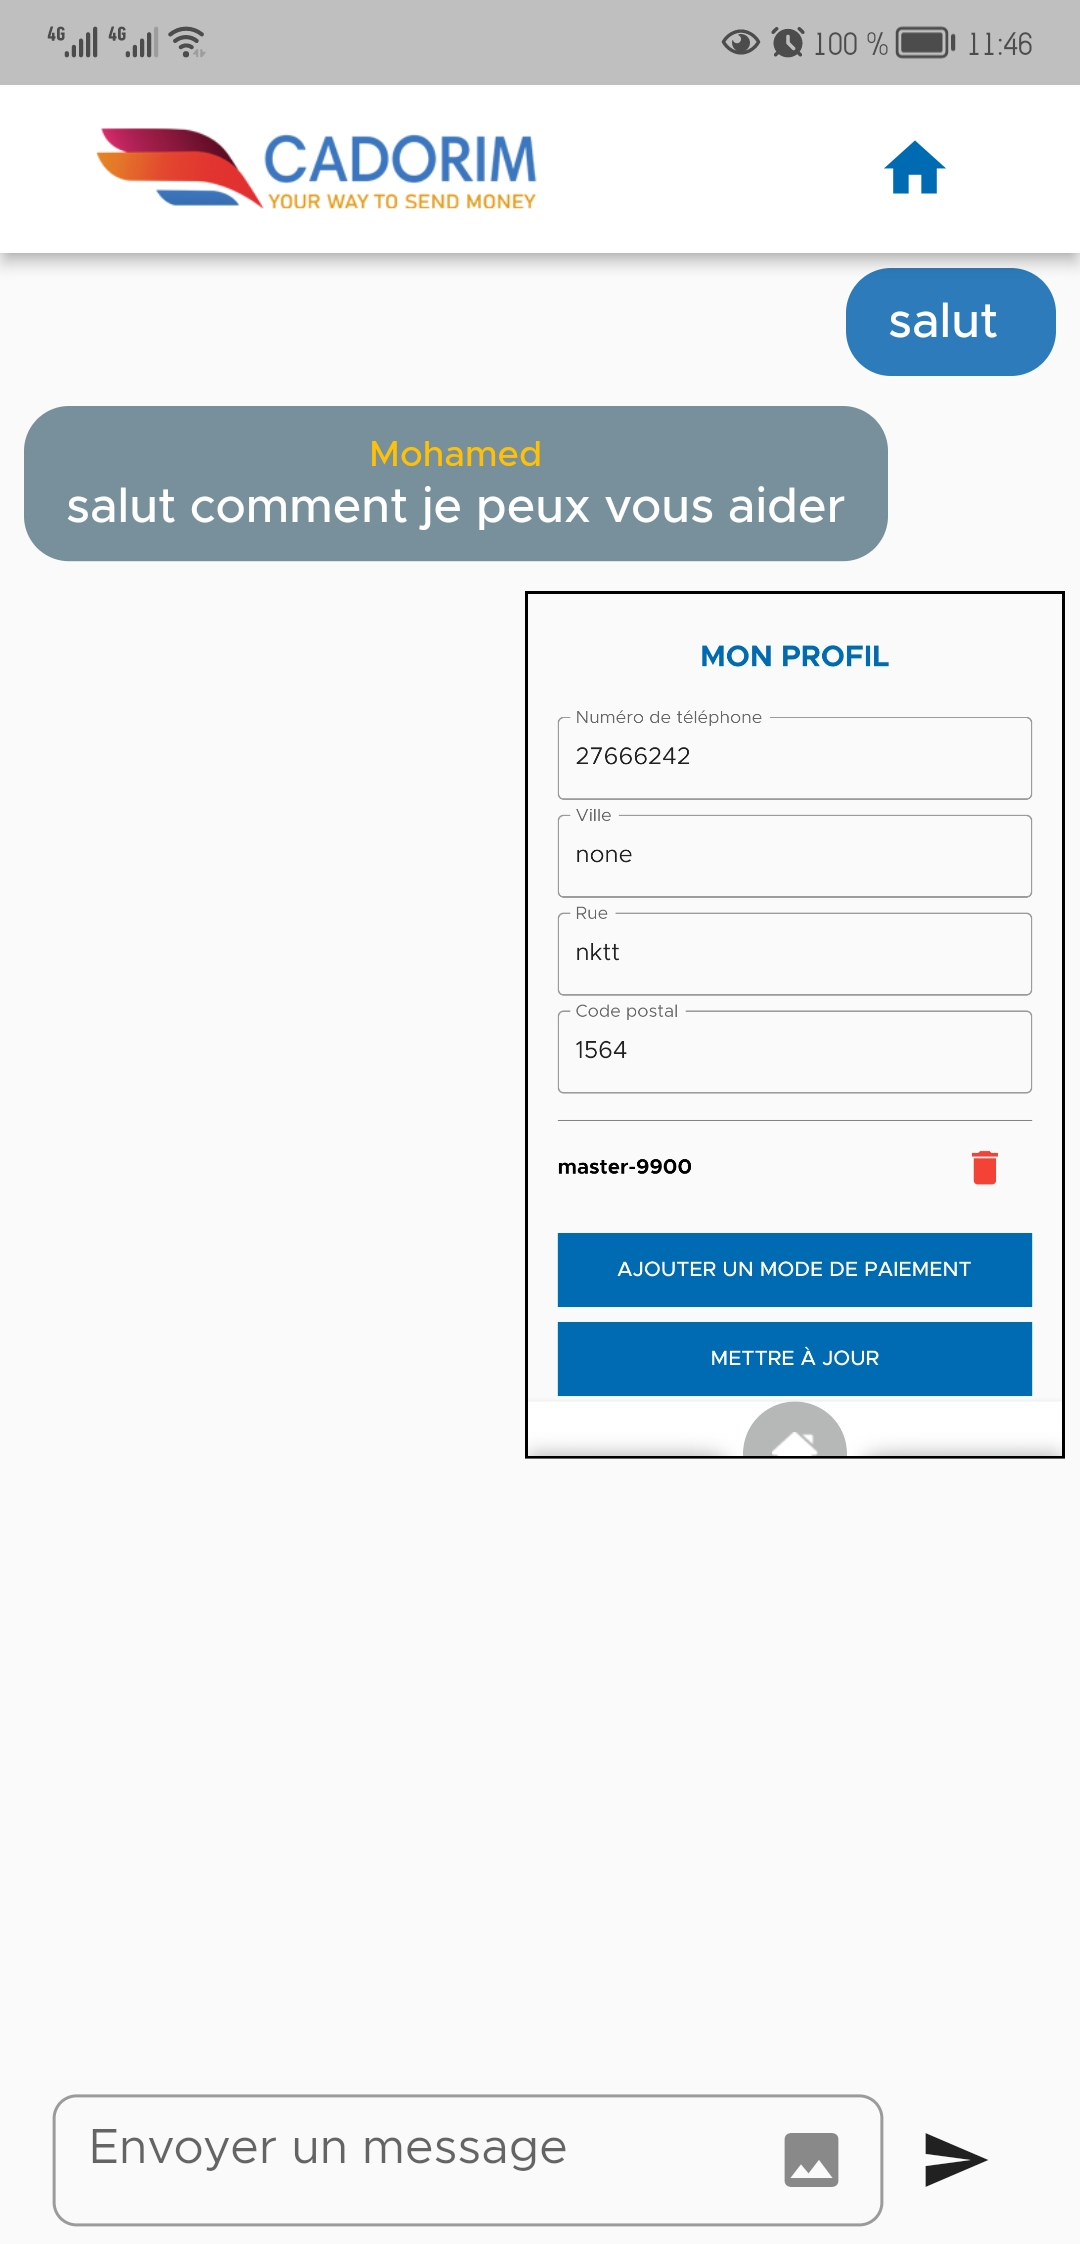
\includegraphics[width=5cm]{./Template LaTeX/Images/c.jpg} }}%
		\caption{Interface de discussion}%
		\label{fig:example}%
	\end{figure}
	\newpage
	\item \textbf{Profil de l'utilisateur:} L'utilisateur peut mettre à jour leur profil ou ajouter un mode paiement comme il montre la figure suivante
	\begin{figure}
		\centering
		\begin{subfigure}[b]{0.3\textwidth}
			\centering
			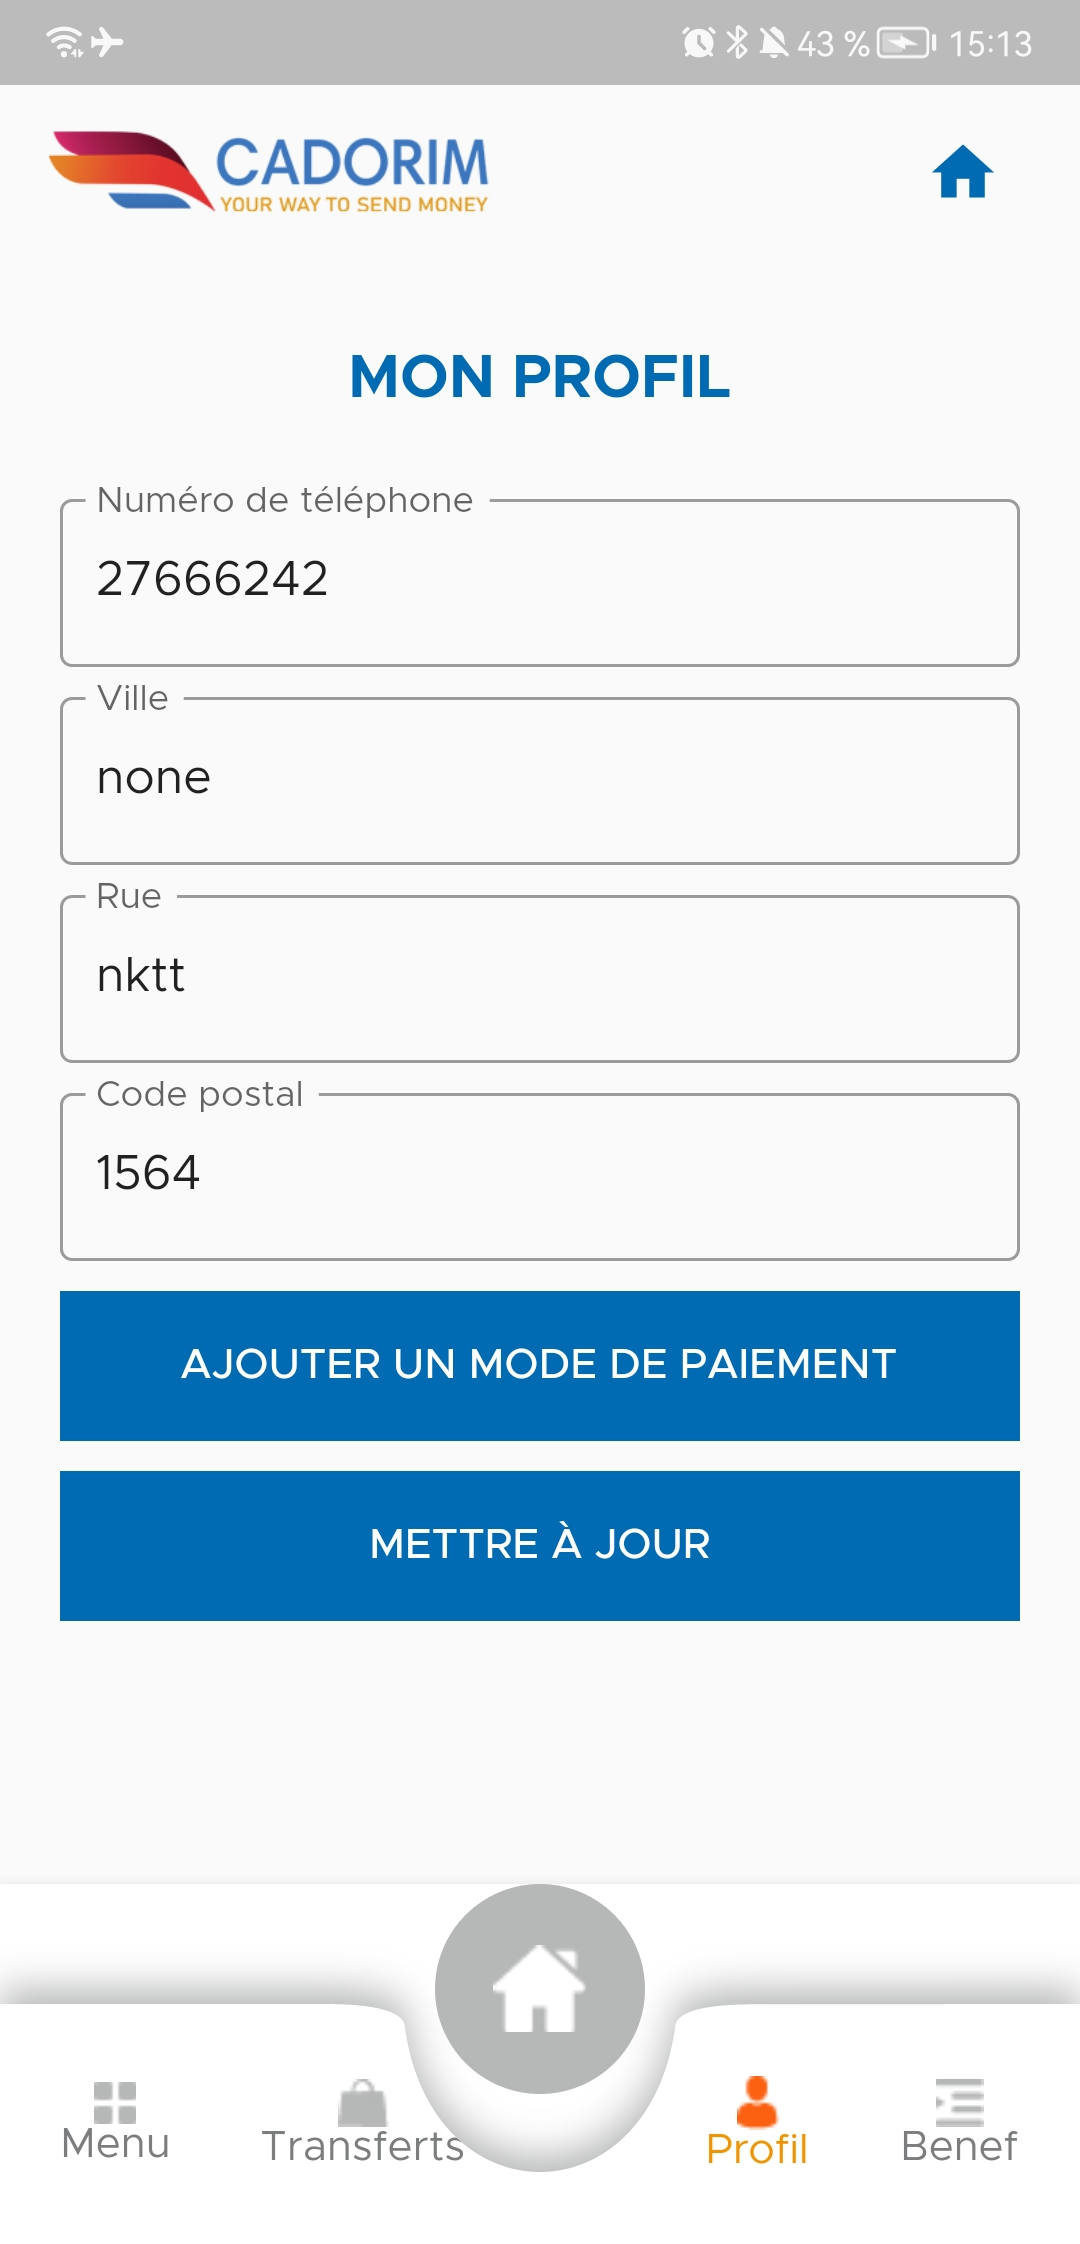
\includegraphics[width=\textwidth]{./Template LaTeX/Images/6.jpg}
			\caption{Mon profil}
			\label{fig:y equals x}
		\end{subfigure}
		\hfill
		\begin{subfigure}[b]{0.3\textwidth}
			\centering
			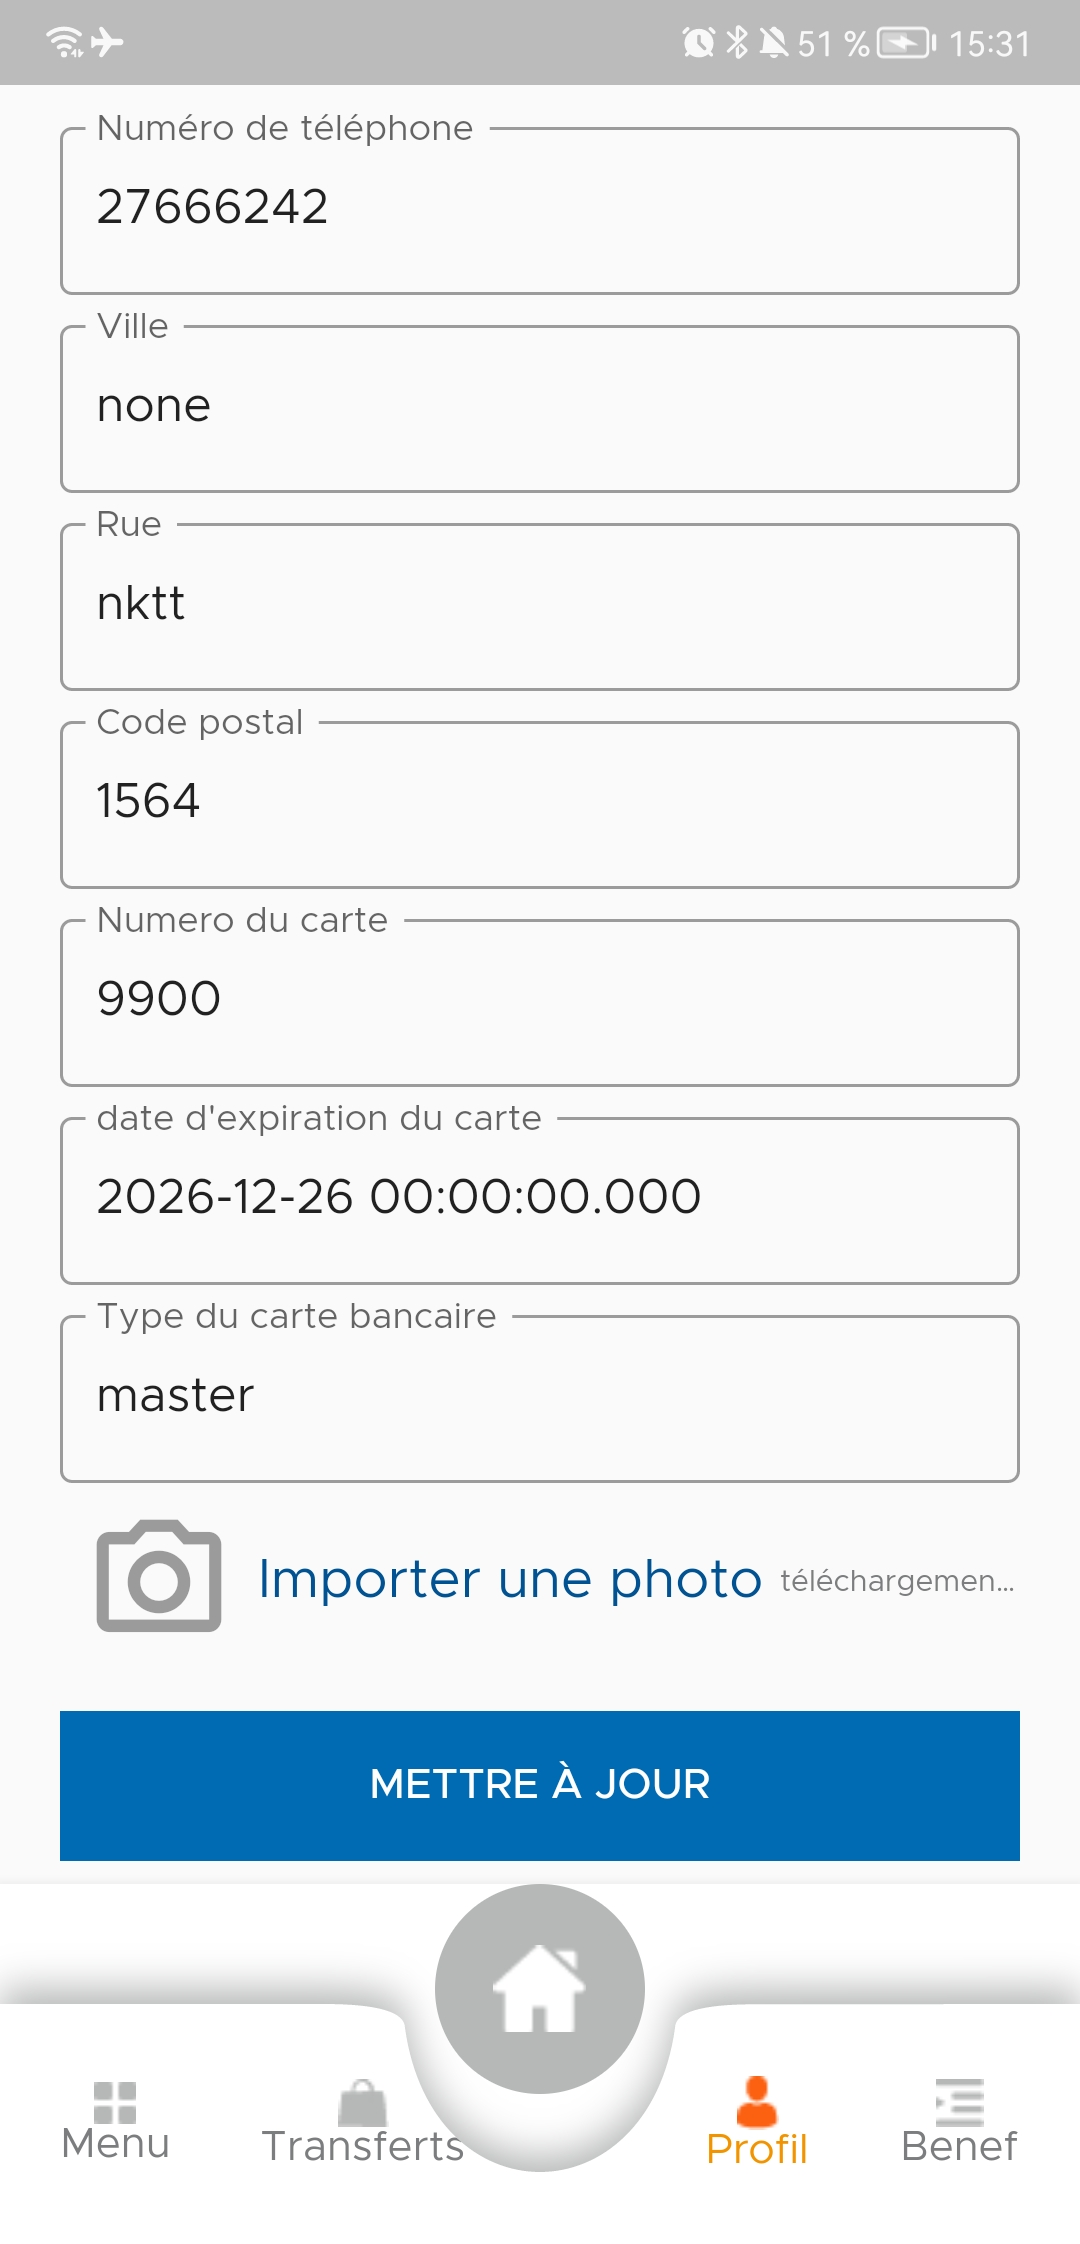
\includegraphics[width=\textwidth]{./Template LaTeX/Images/7.jpg}
			\caption{Ajouter une carte}
			\label{fig:three sin x}
		\end{subfigure}
		\hfill
		\begin{subfigure}[b]{0.3\textwidth}
			\centering
			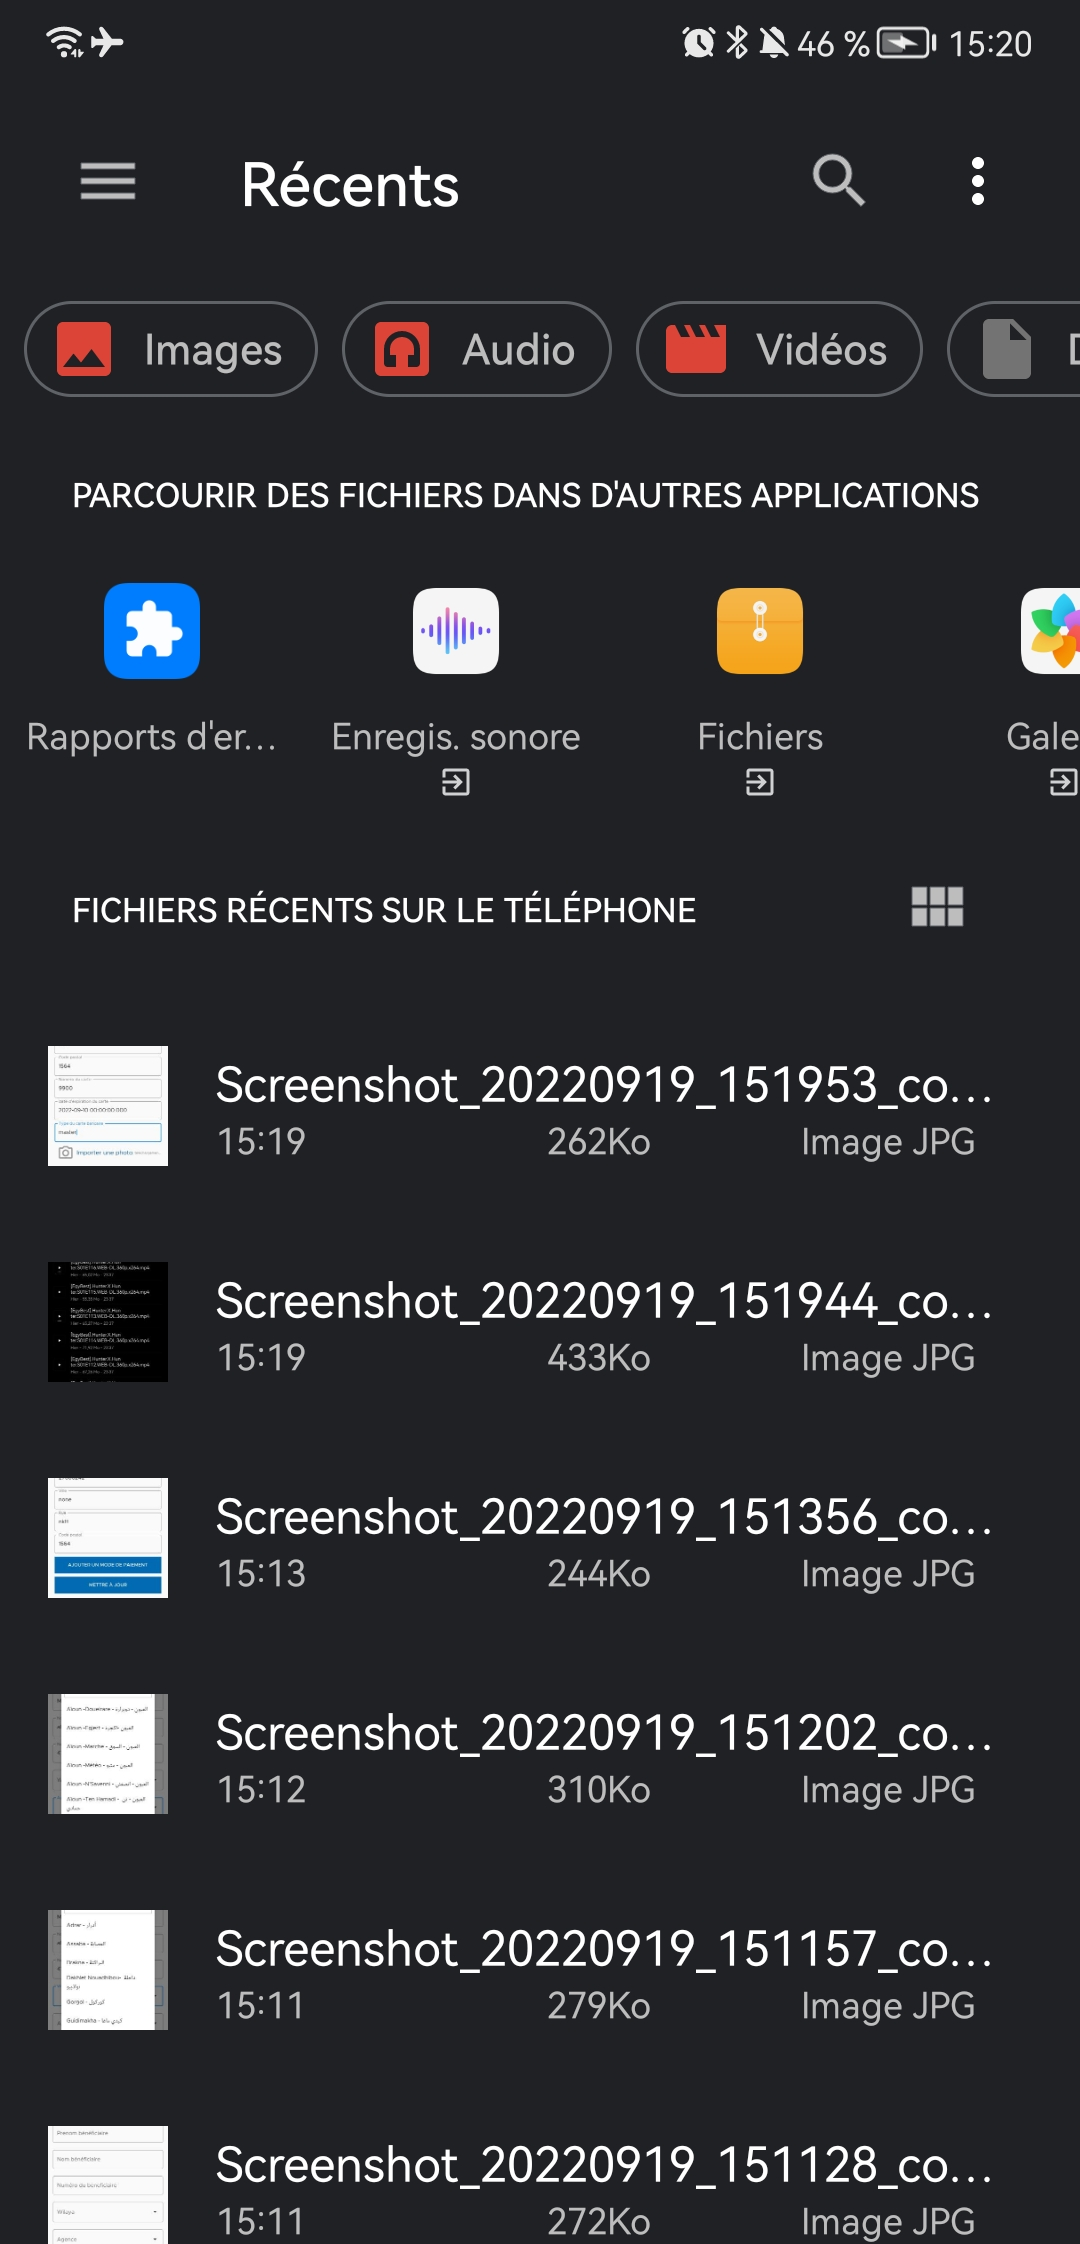
\includegraphics[width=\textwidth]{./Template LaTeX/Images/8.jpg}
			\caption{Importer une photo}
			\label{fig:five over x}
		\end{subfigure}
		\newline
		\centering
		\begin{subfigure}{0.3\textwidth}
			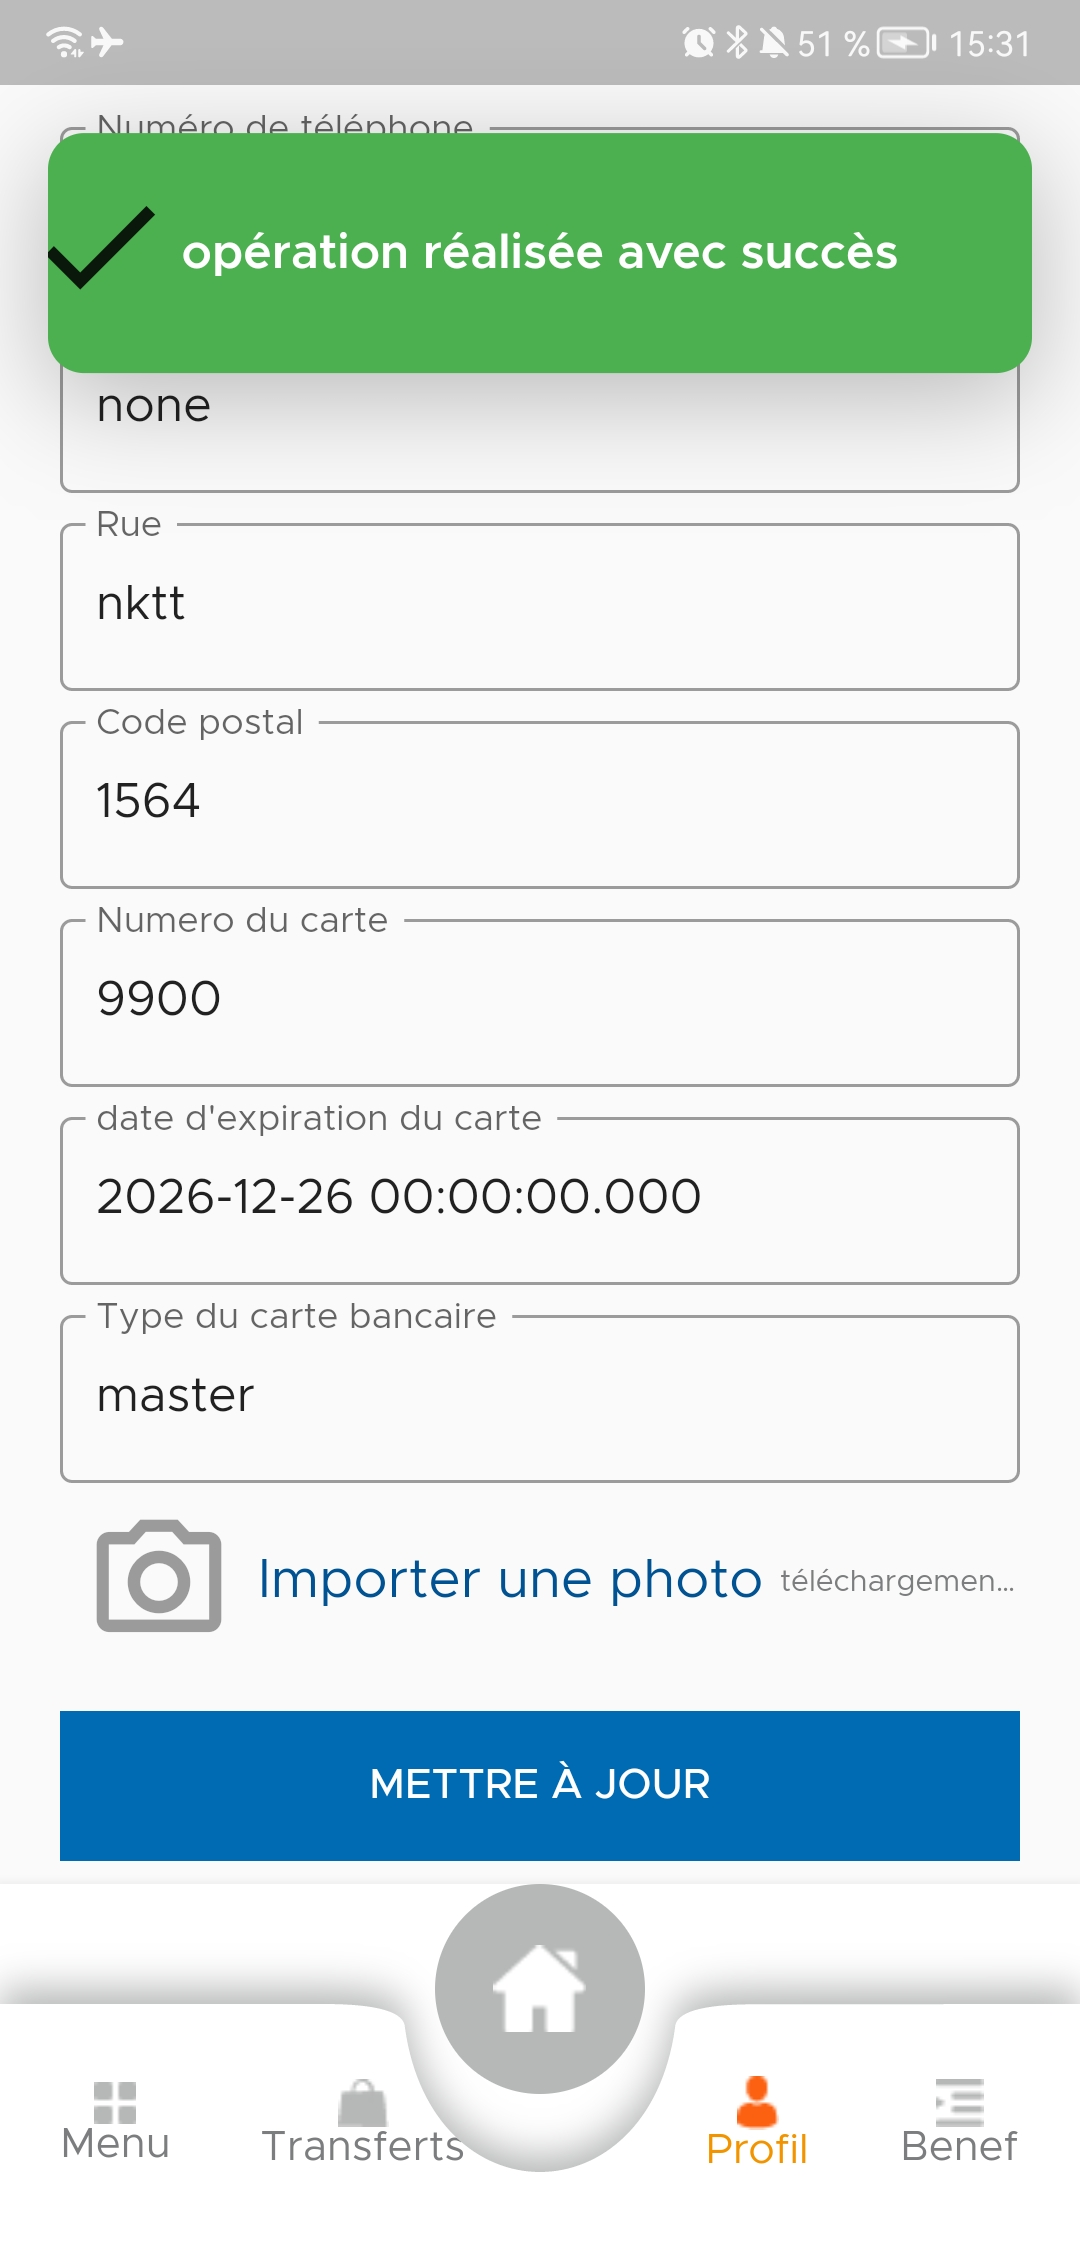
\includegraphics[width=\hsize, valign=m ]{./Template LaTeX/Images/9.jpg}
			\caption{État}
			\label{fig.SICAPI}
		\end{subfigure}
		%\qquad\tikz[baseline=-\baselineskip]\draw[ultra thick,->] (0,0) -- ++ (1,0);\qquad
		\begin{subfigure}{0.3\textwidth}
			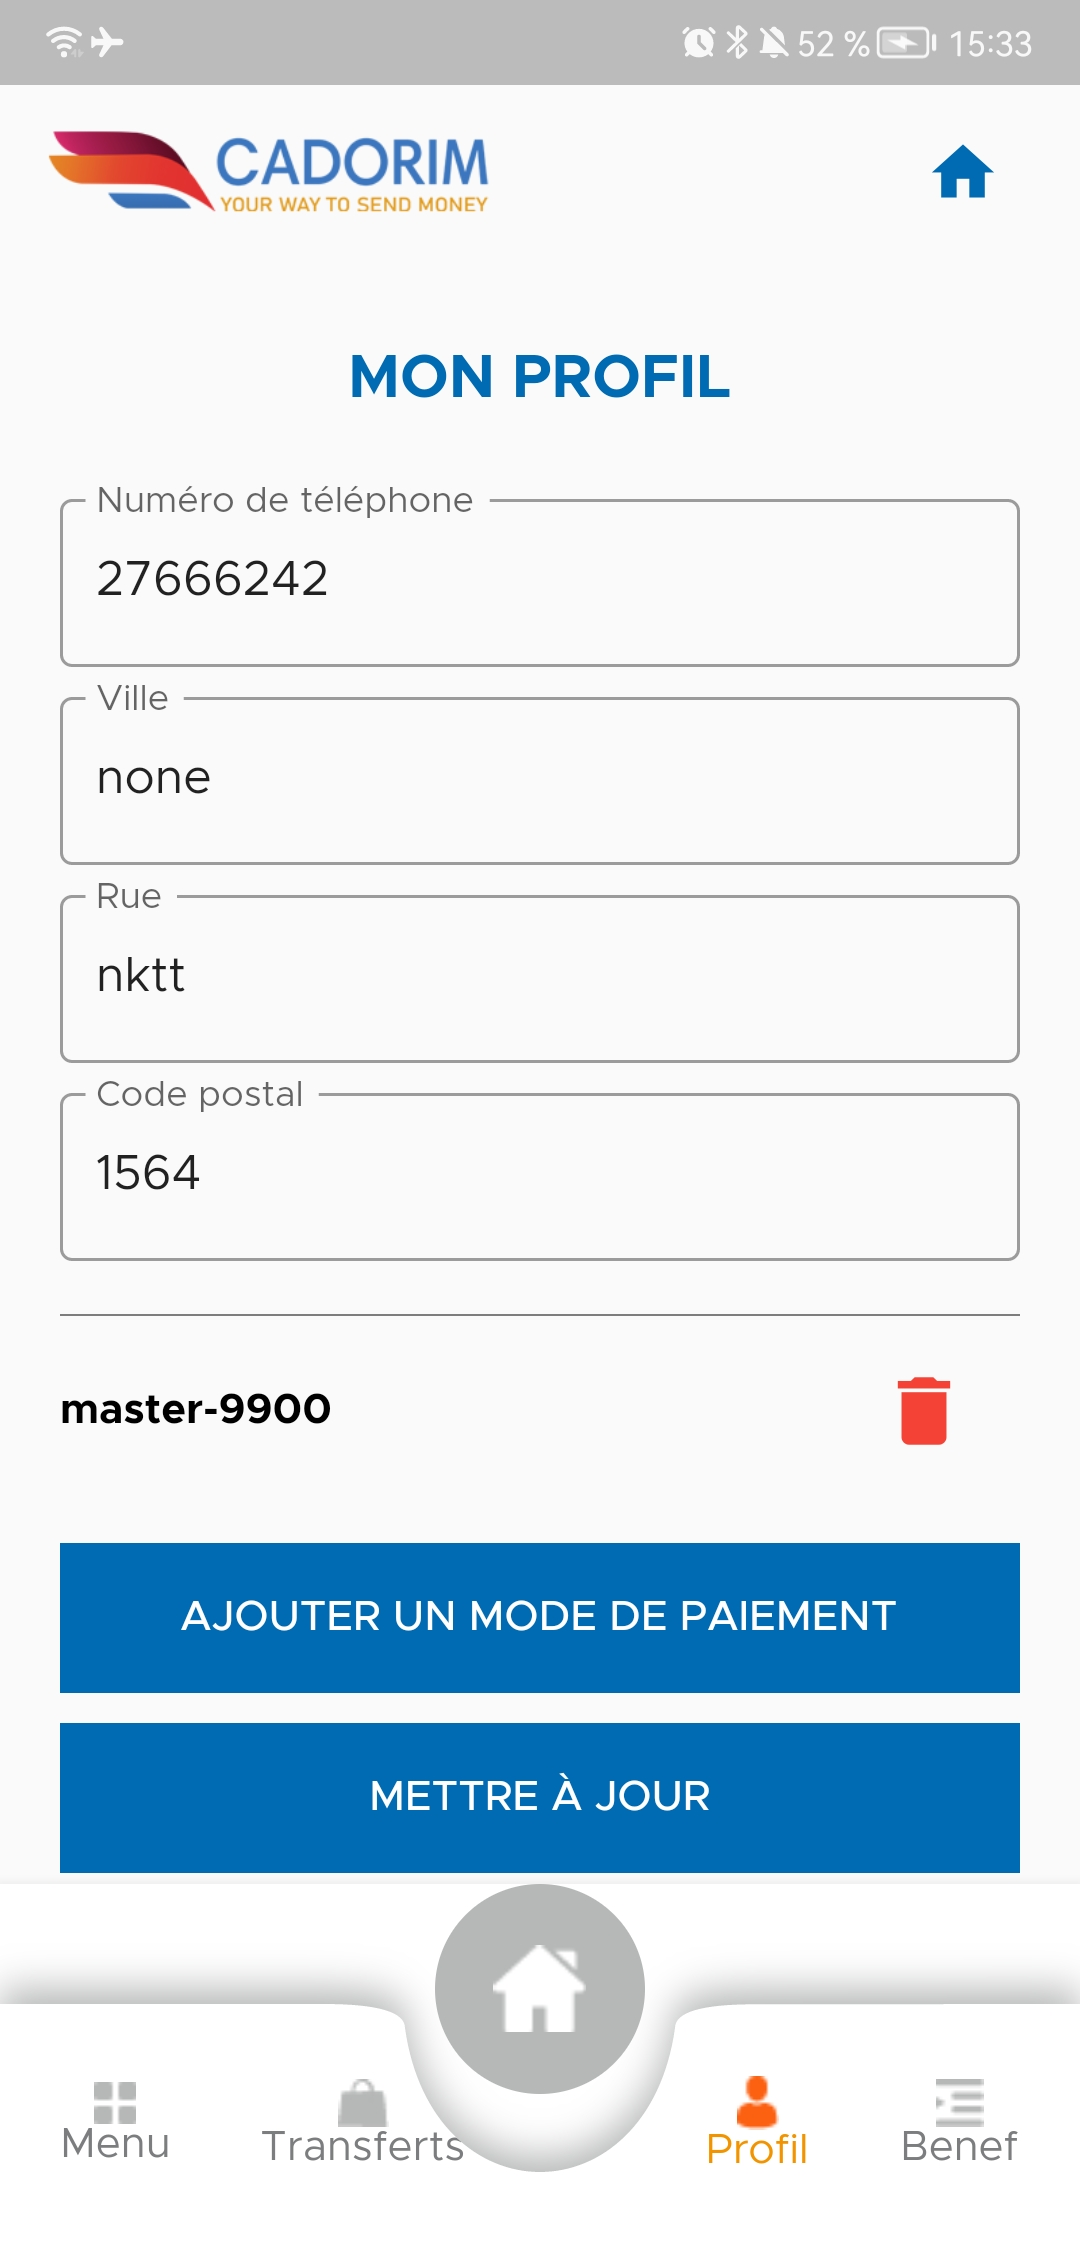
\includegraphics[width=\hsize, valign=m]{./Template LaTeX/Images/10.jpg}
			\caption{Interface suivante}
			\label{fig.painel_sicapi}
		\end{subfigure}
		\caption{Profil de l'utilisateur
		}
		\label{fig:three graphs}
	\end{figure}
	
	
	%%%%%%%%%%%%%%%%%%%%%%%%%%%%%%%%MENU%%%%%%%%%%%%%%%%%%%%%%%%%%%%%%%
	\newpage
	\item \textbf{L’interface de menu
		:} À partir de cette fenêtre le client a l'accès aux autres fonctionalistes de l'application (Modifier mot de passe,changer la langue ....)
	\begin{figure}%
		\centering
		{{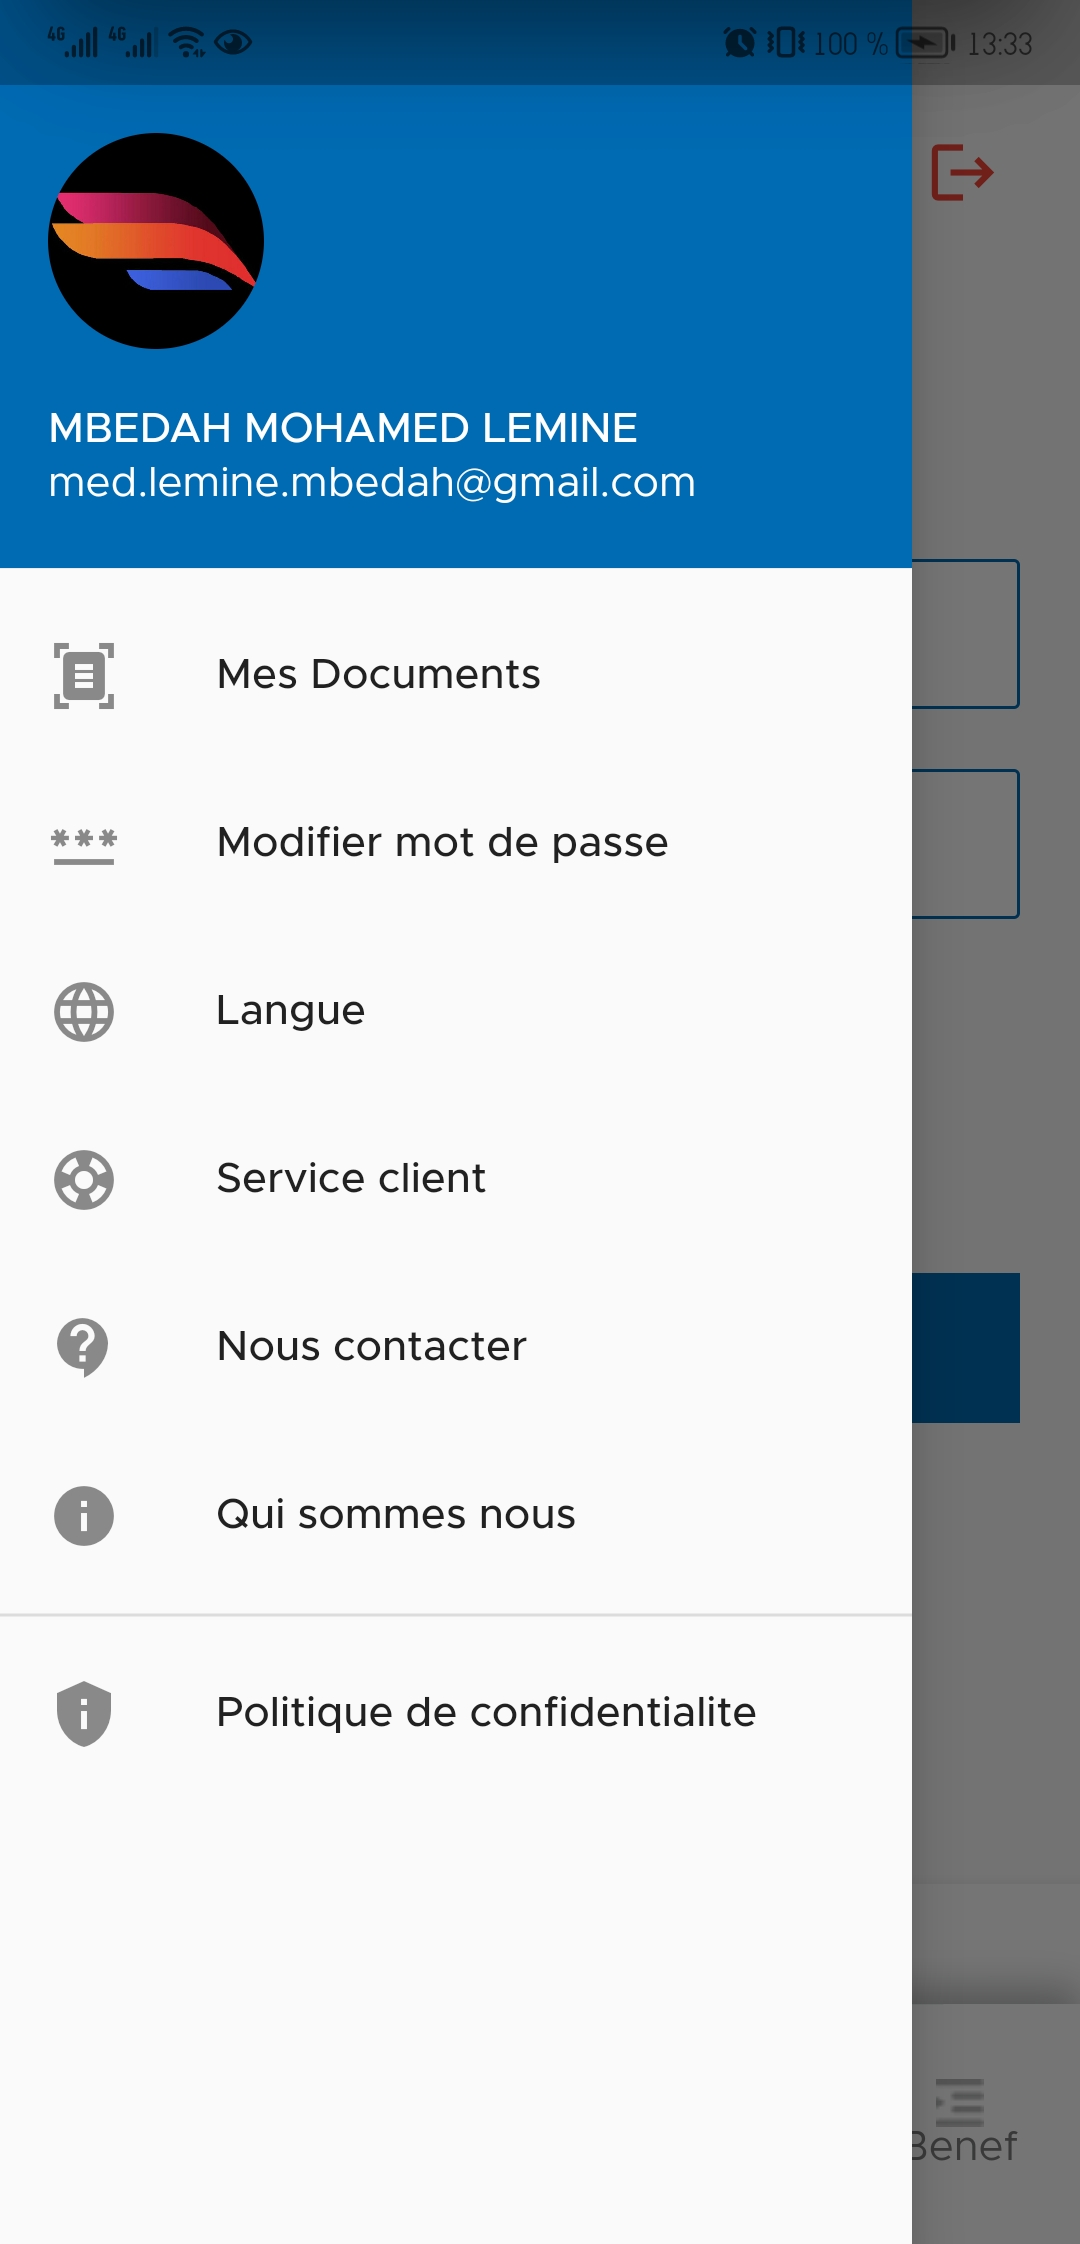
\includegraphics[width=5cm]{./Template LaTeX/Images/menu.jpg} }}%
		\caption{Interface de menu}%
		\label{fig:example}%
	\end{figure}
\end{itemize}

\subsubsection{Application ServiceClient}
\begin{itemize}[label=$\ast$]
	\item \textbf{L’interface
		d’authentification
		:} La figure suivante représente l’interface d’authentification de notre application. Elle permet aux utilisateurs de s’identifier en introduisant leurs identifiants afin d’accéder aux fonctionnalités de l’application.
	
	\begin{figure}%
		\centering
		{{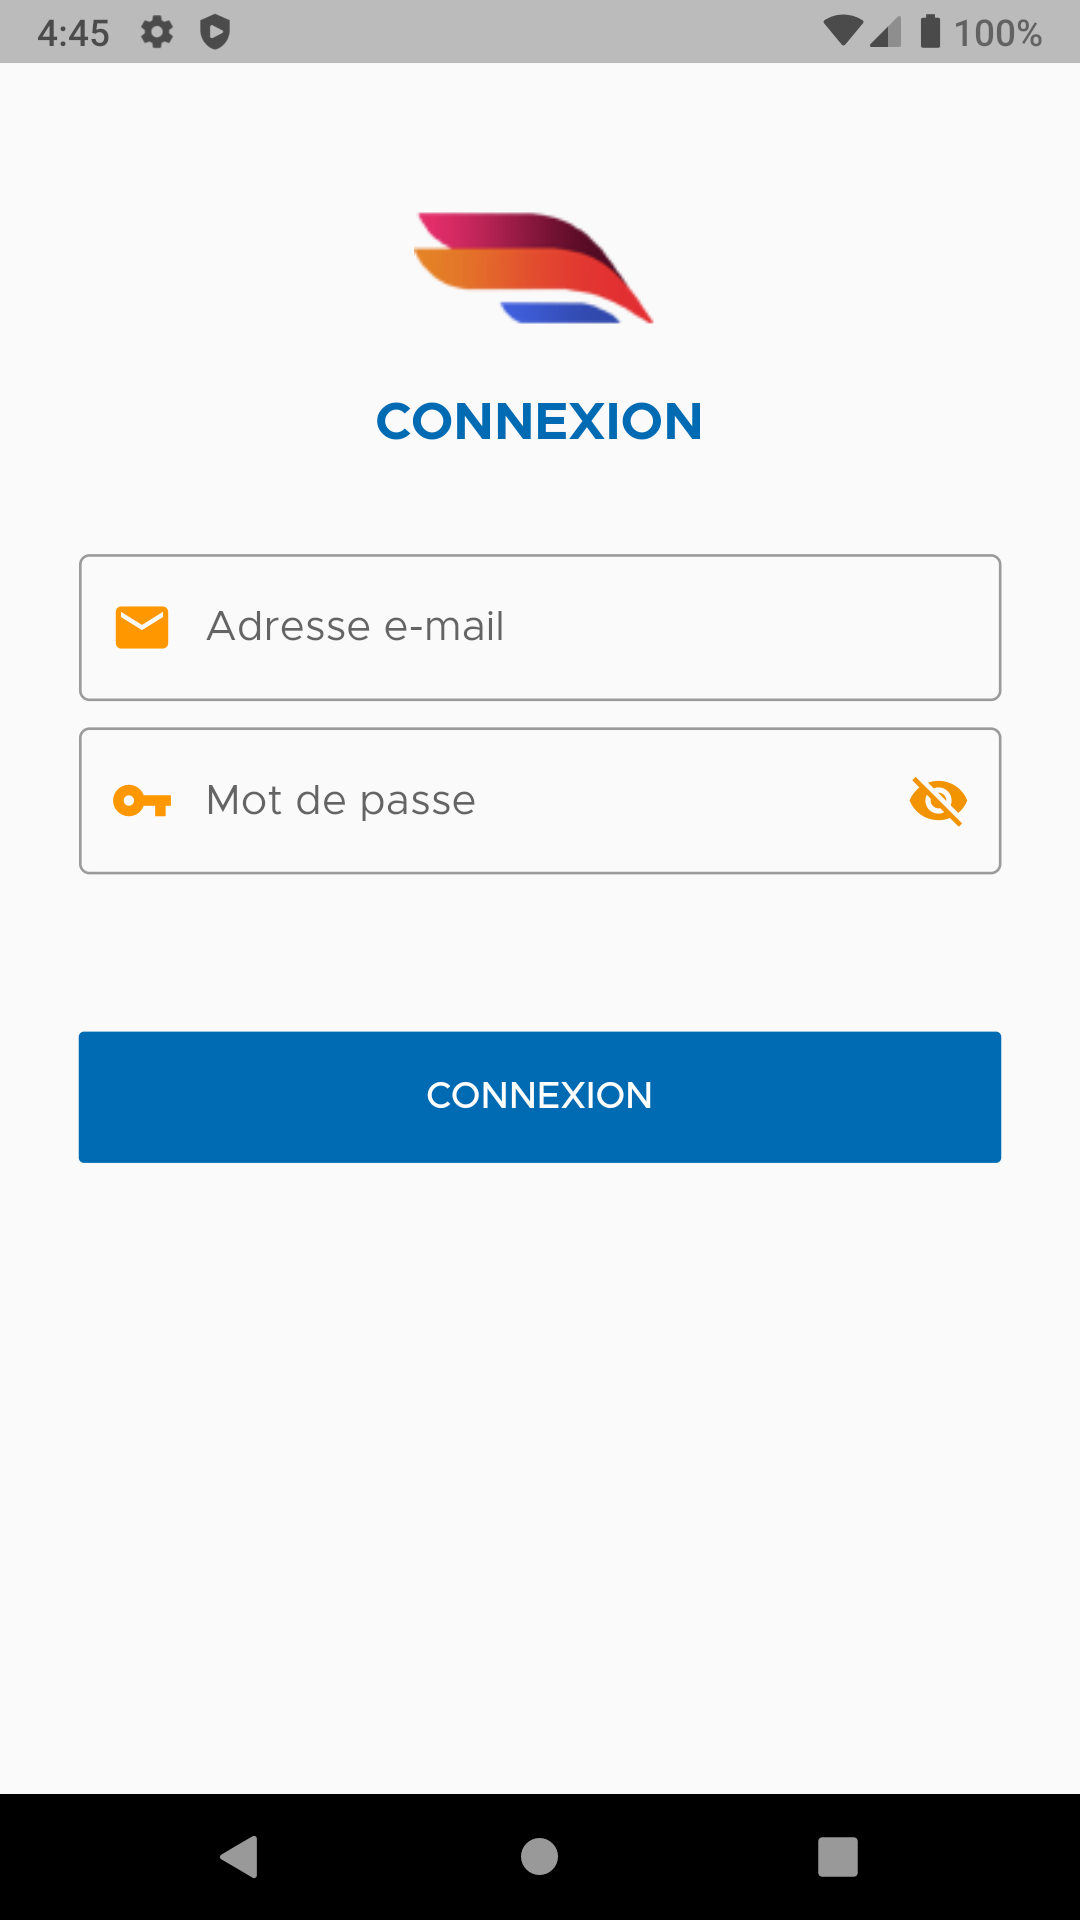
\includegraphics[width=5cm]{./Template LaTeX/Images/From_emu/login.png} }}%
		\caption{Interface d'authentification}%
		\label{fig:example}%
	\end{figure}
	\newpage
	\item \textbf{L’interface du compte administrateur
		:} La figure~\ref{Home} représente la page principale de l’application pour l'administrateur. C’est à partir de cette fenêtre qu’est accessible la majorité des fonctionnalités de base de l’application(Gérer les comptes de service client).
	\begin{comment}
		content...
	}
	\begin{figure}
		\centering
		\begin{subfigure}[b]{0.3\textwidth}
			\centering
			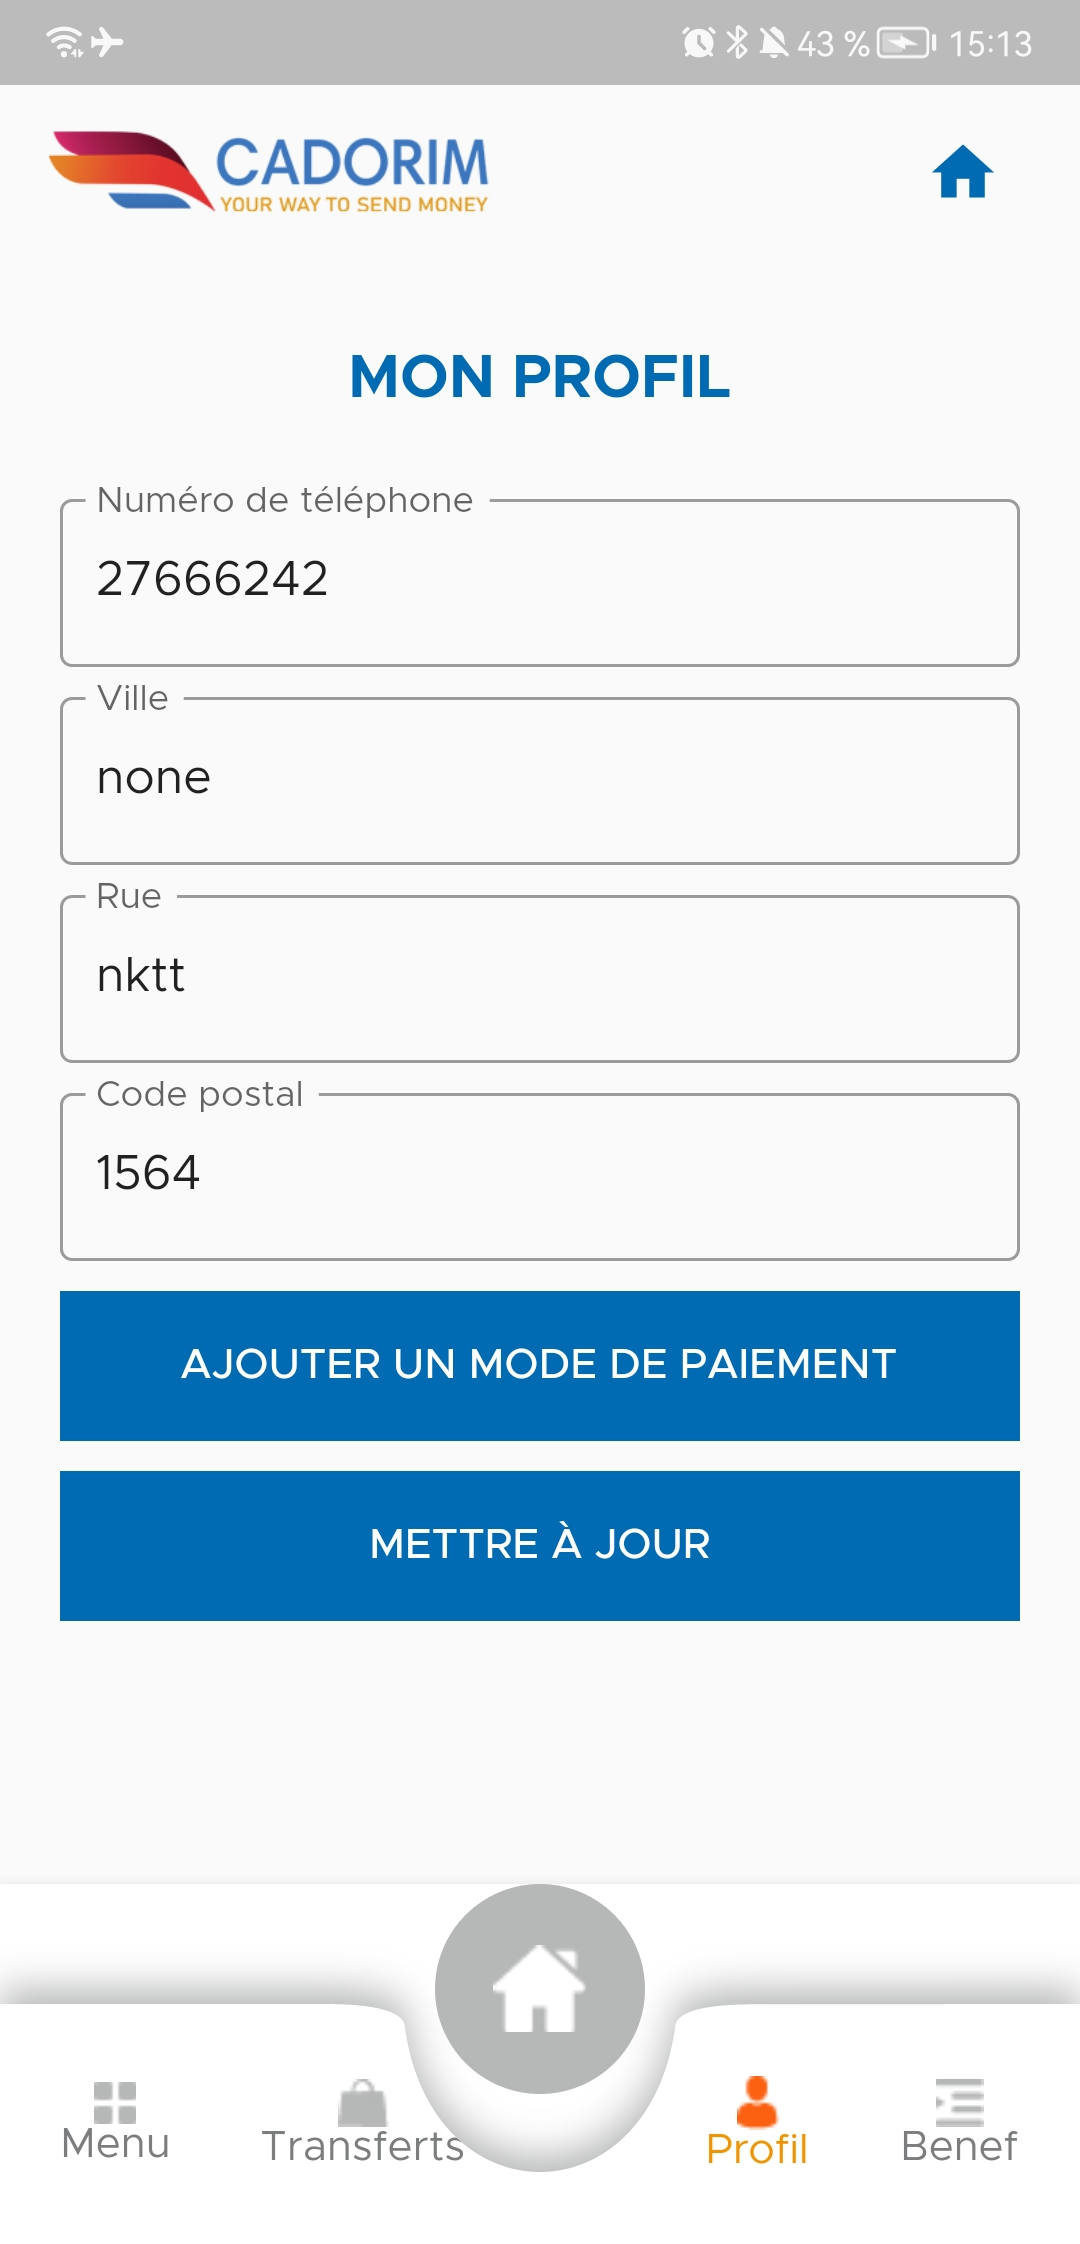
\includegraphics[width=\textwidth]{./Template LaTeX/Images/6.jpg}
			\caption{Interfaces d’accueil}
			\label{fig:y equals x}
		\end{subfigure}
		\hfill
		\begin{subfigure}[b]{0.3\textwidth}
			\centering
			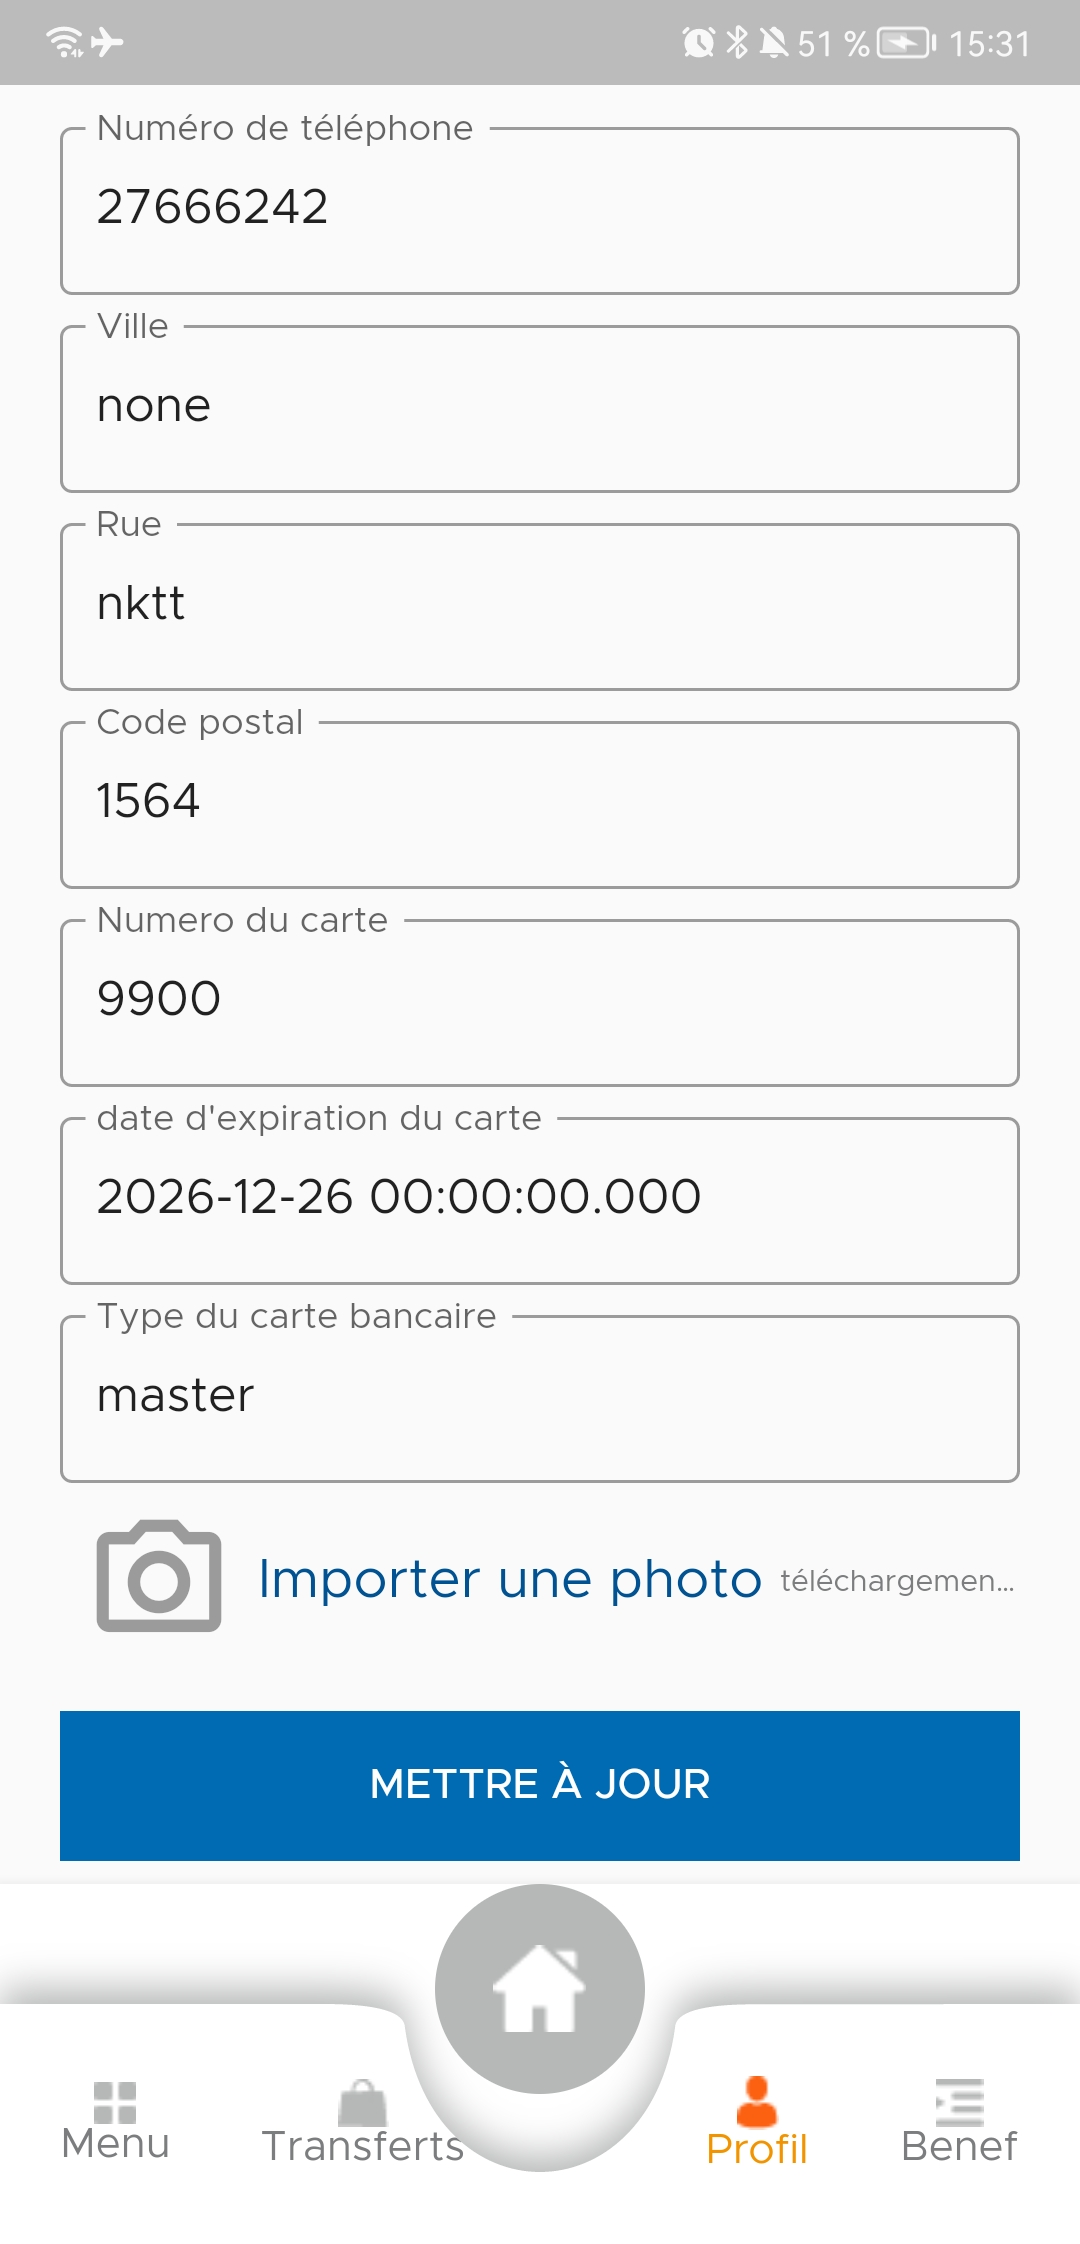
\includegraphics[width=\textwidth]{./Template LaTeX/Images/7.jpg}
			\caption{Supprimer un compte}
			\label{fig:three sin x}
		\end{subfigure}
		\hfill
		\begin{subfigure}[b]{0.3\textwidth}
			\centering
			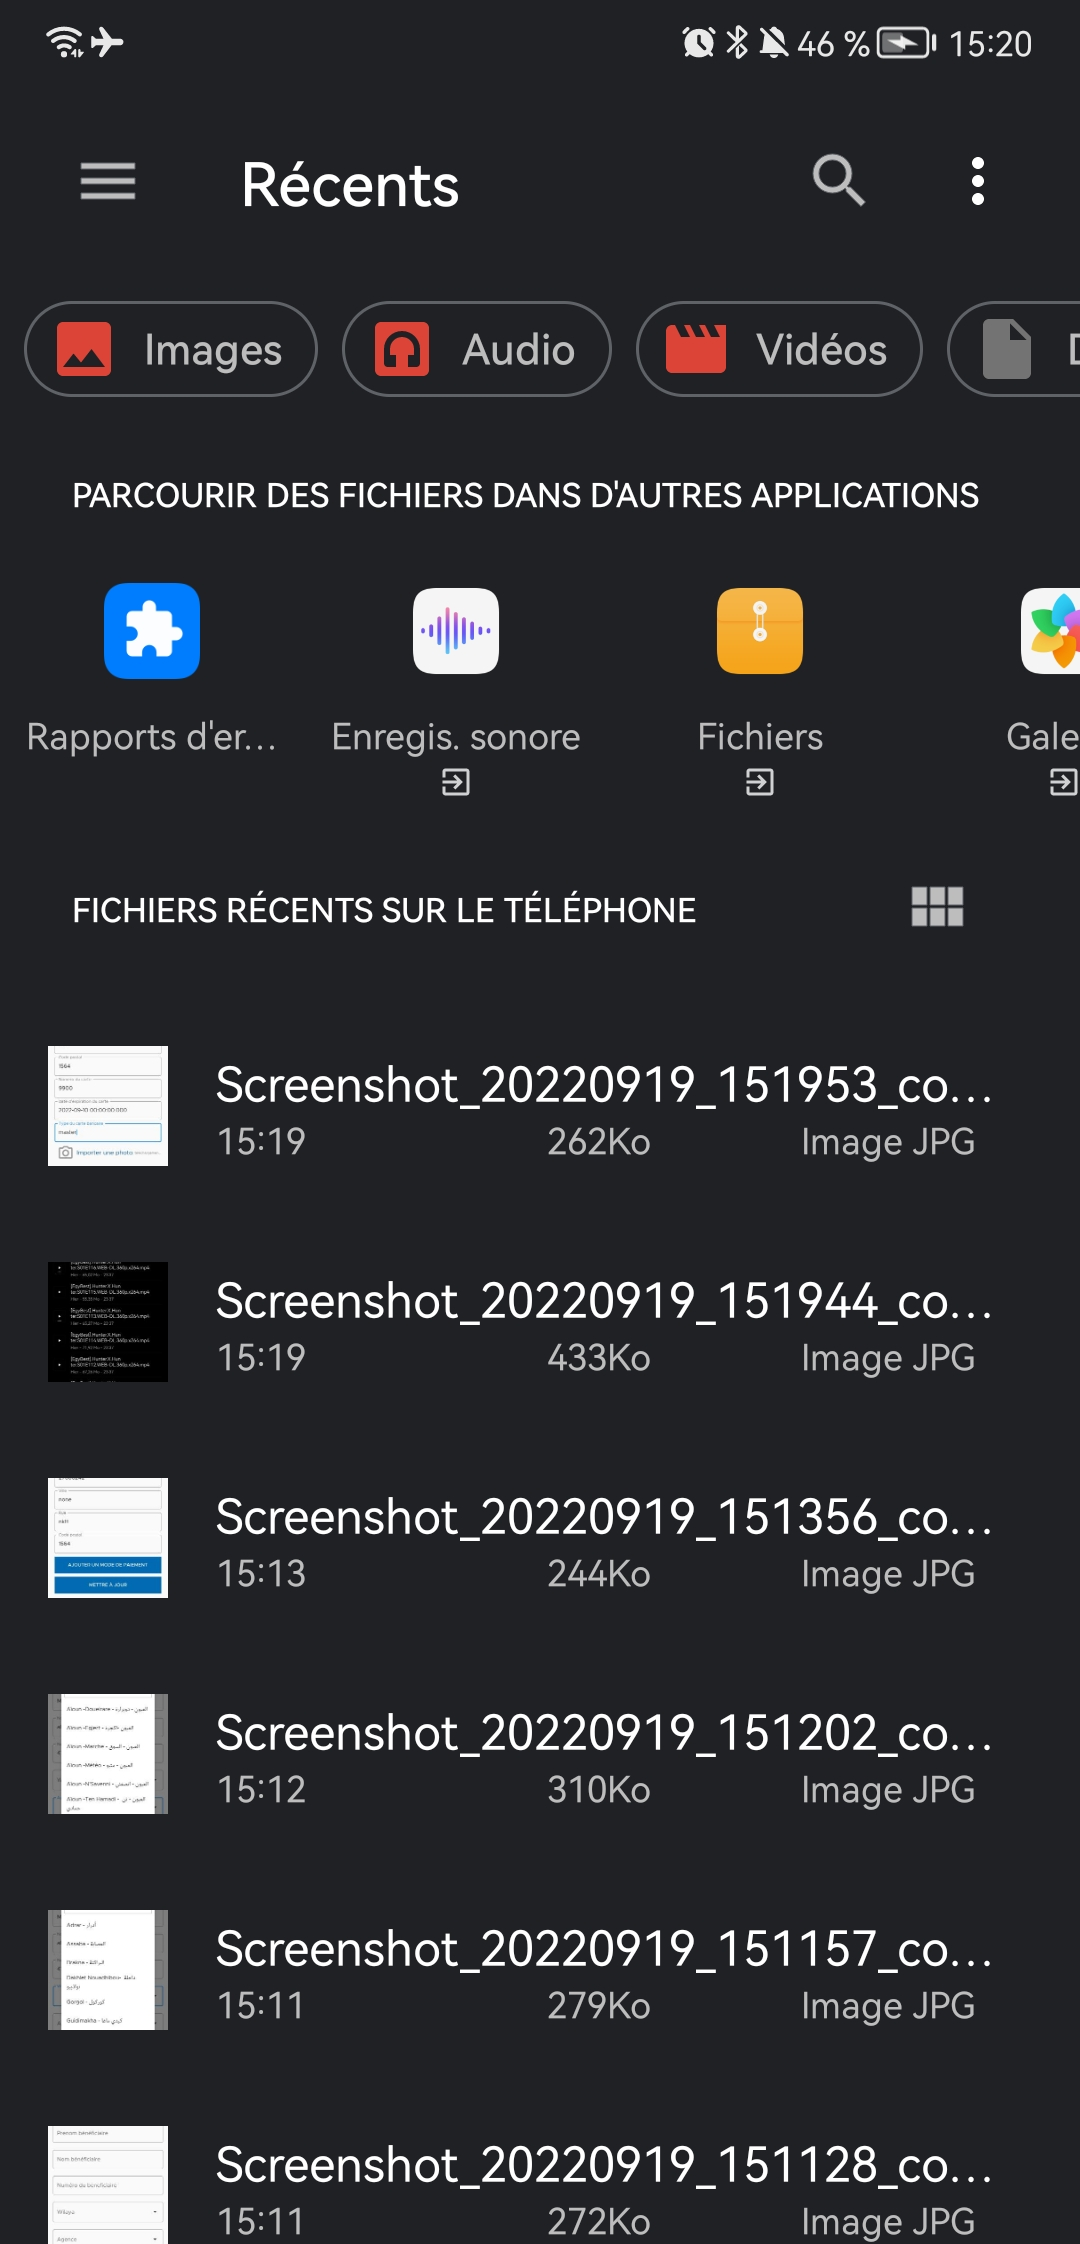
\includegraphics[width=\textwidth]{./Template LaTeX/Images/8.jpg}
			\caption{Mettre à jour un compte}
			\label{fig:five over x}
		\end{subfigure}
		\caption{Interface du compte principal
		}
		\label{Home}
	\end{figure}
\end{comment}
%%%%%%%%%%%%%%%%%%%%%%%%%%%%%%%%%%%%%%%%%%%%%%%%%%%%%%%%%%%%%
\begin{figure}
	\centering
	\begin{subfigure}[b]{0.3\textwidth}
		\centering
		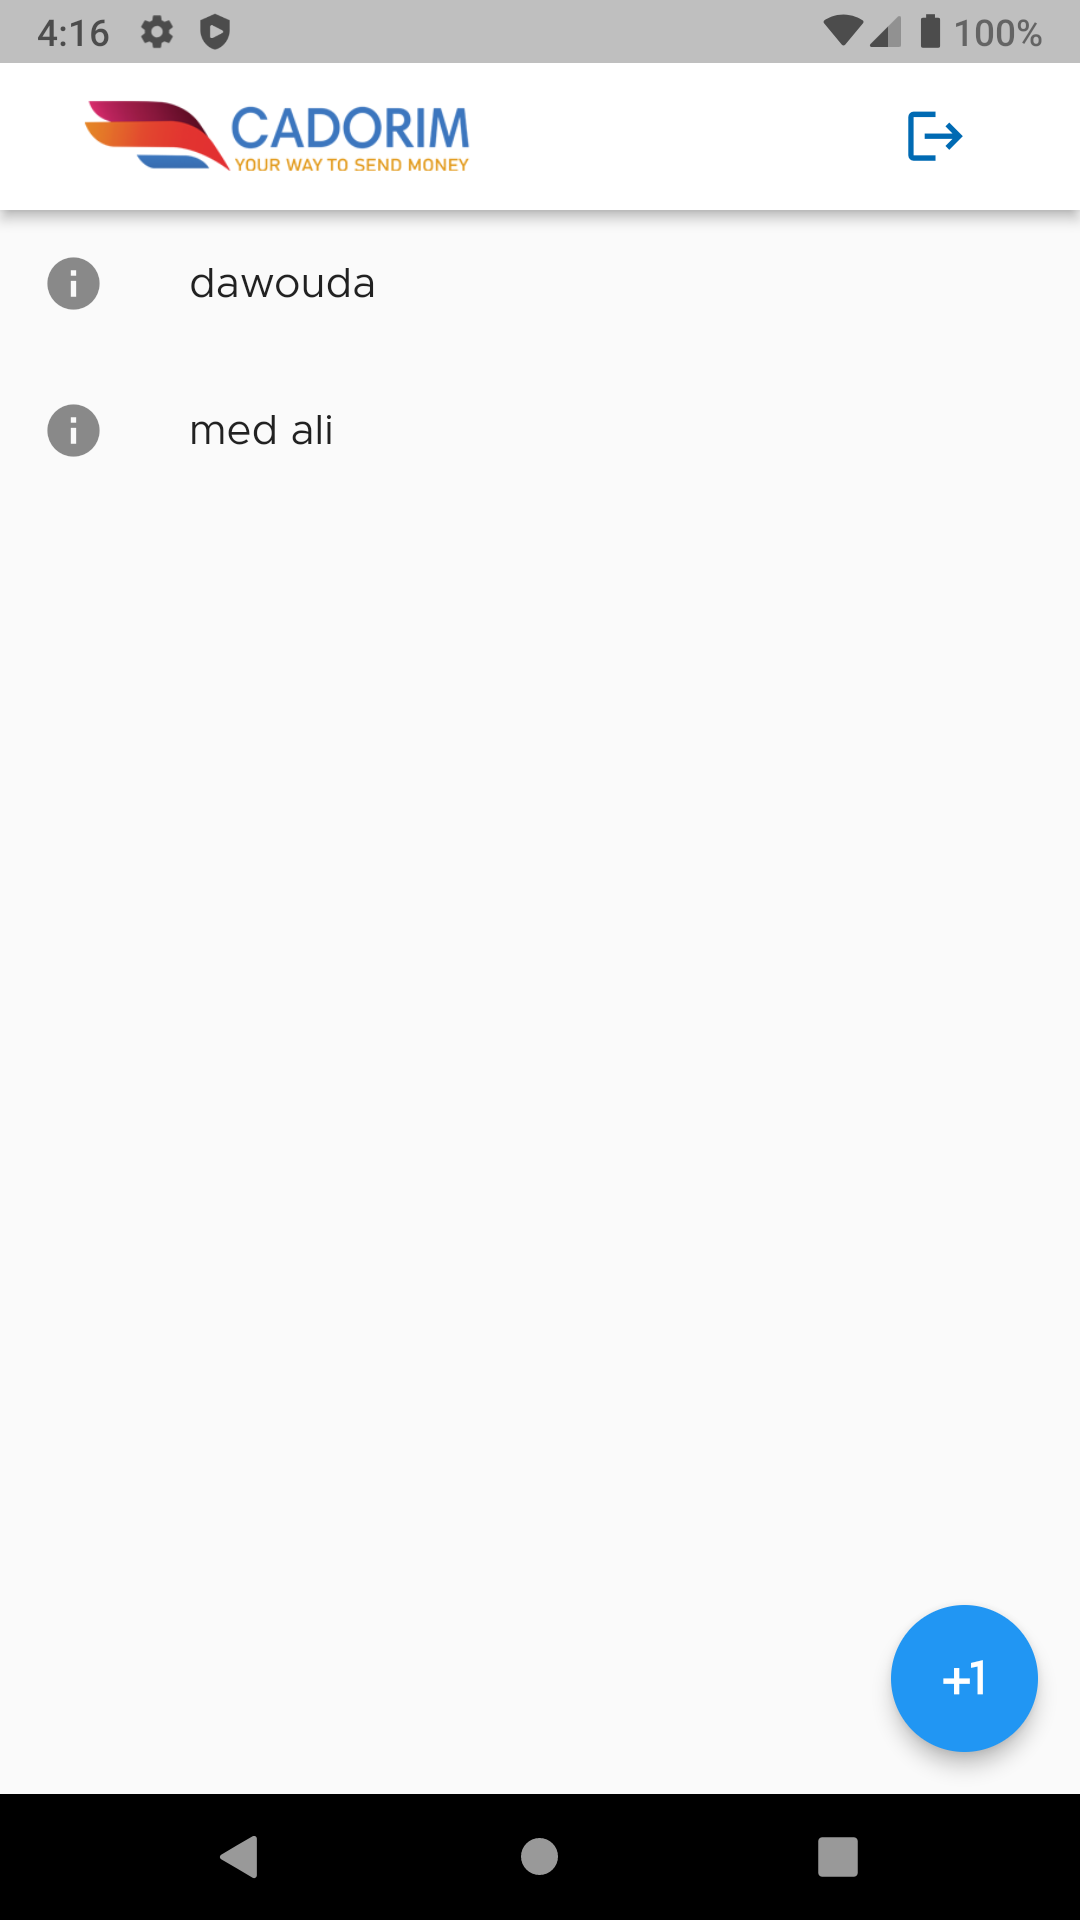
\includegraphics[width=\textwidth]{./Template LaTeX/Images/From_emu/A_home.png}
		\caption{Interfaces d’accueil}
		\label{fig:y equals x}
	\end{subfigure}
	\hfill
	\begin{subfigure}[b]{0.3\textwidth}
		\centering
		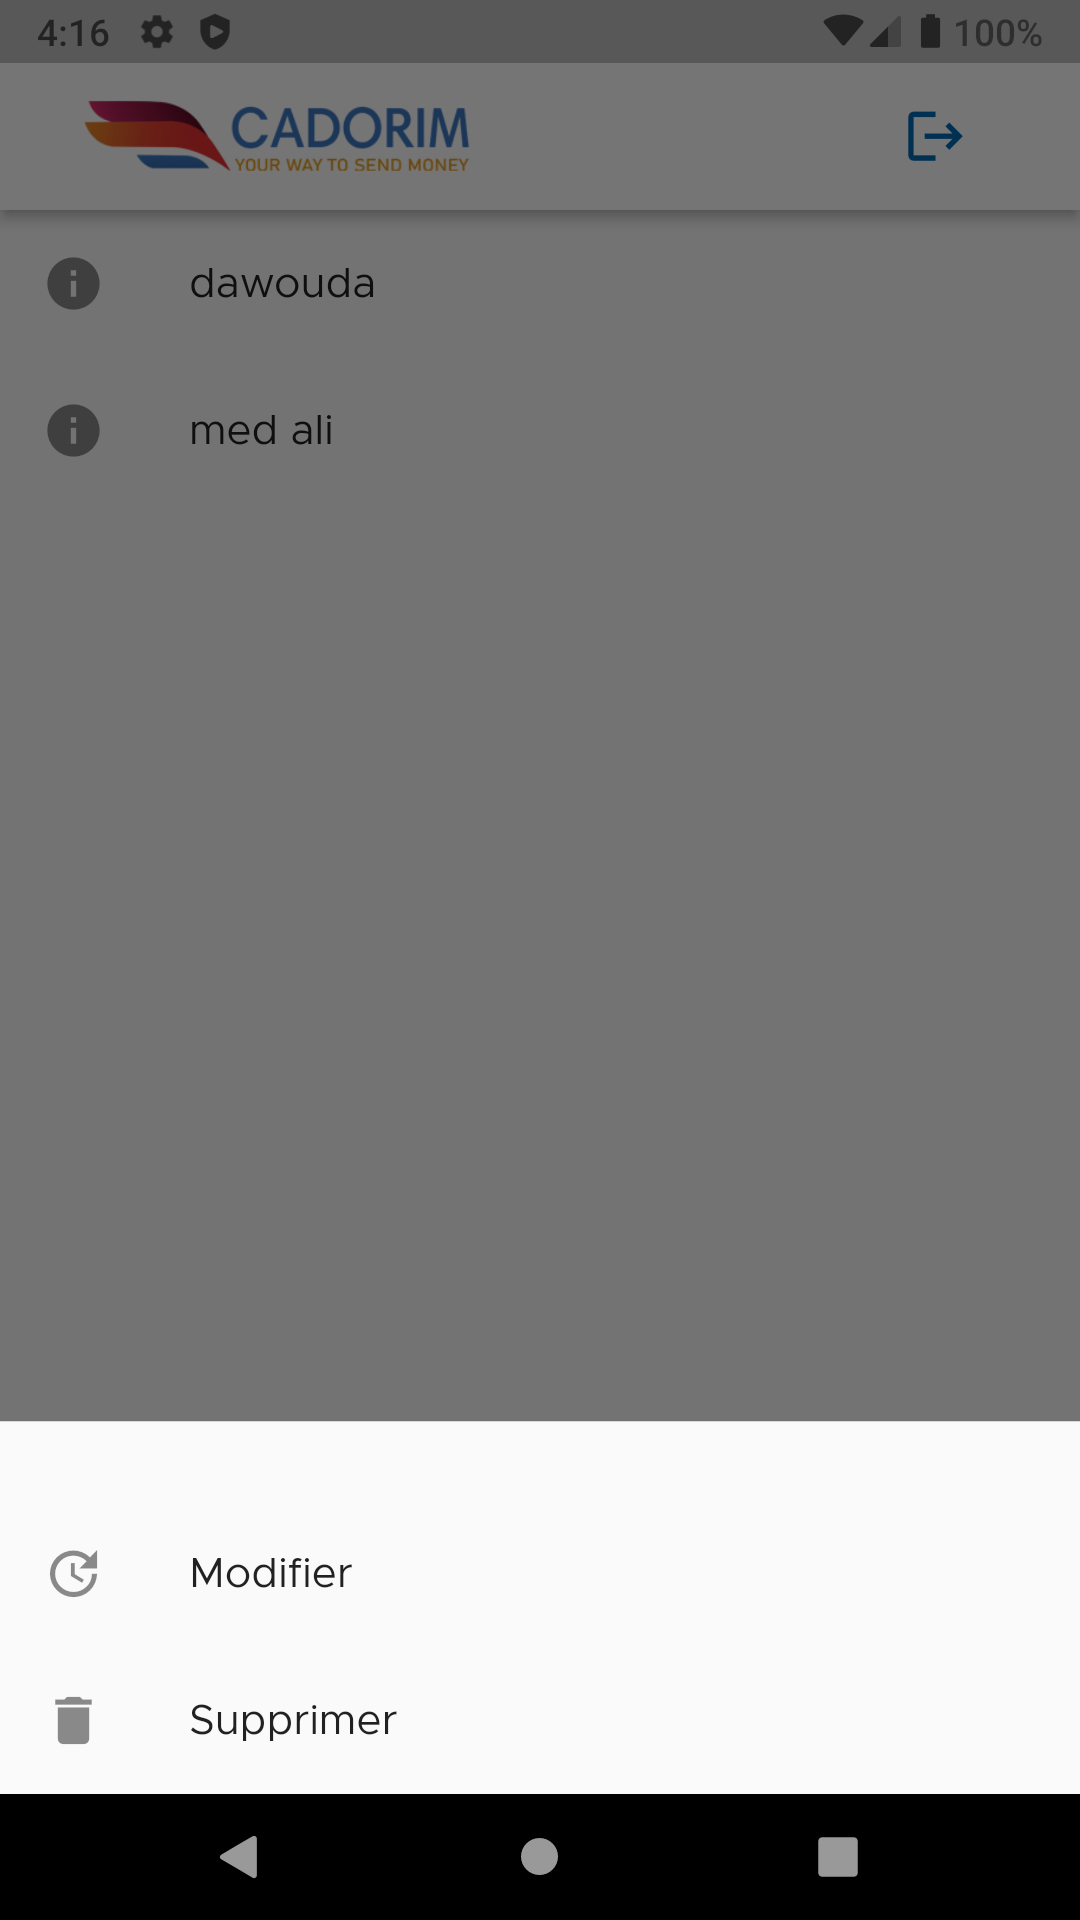
\includegraphics[width=\textwidth]{./Template LaTeX/Images/From_emu/A_update_modif.png}
		\caption{Gérer un compte}
		\label{fig:three sin x}
	\end{subfigure}
	\hfill
	\begin{subfigure}[b]{0.3\textwidth}
		\centering
		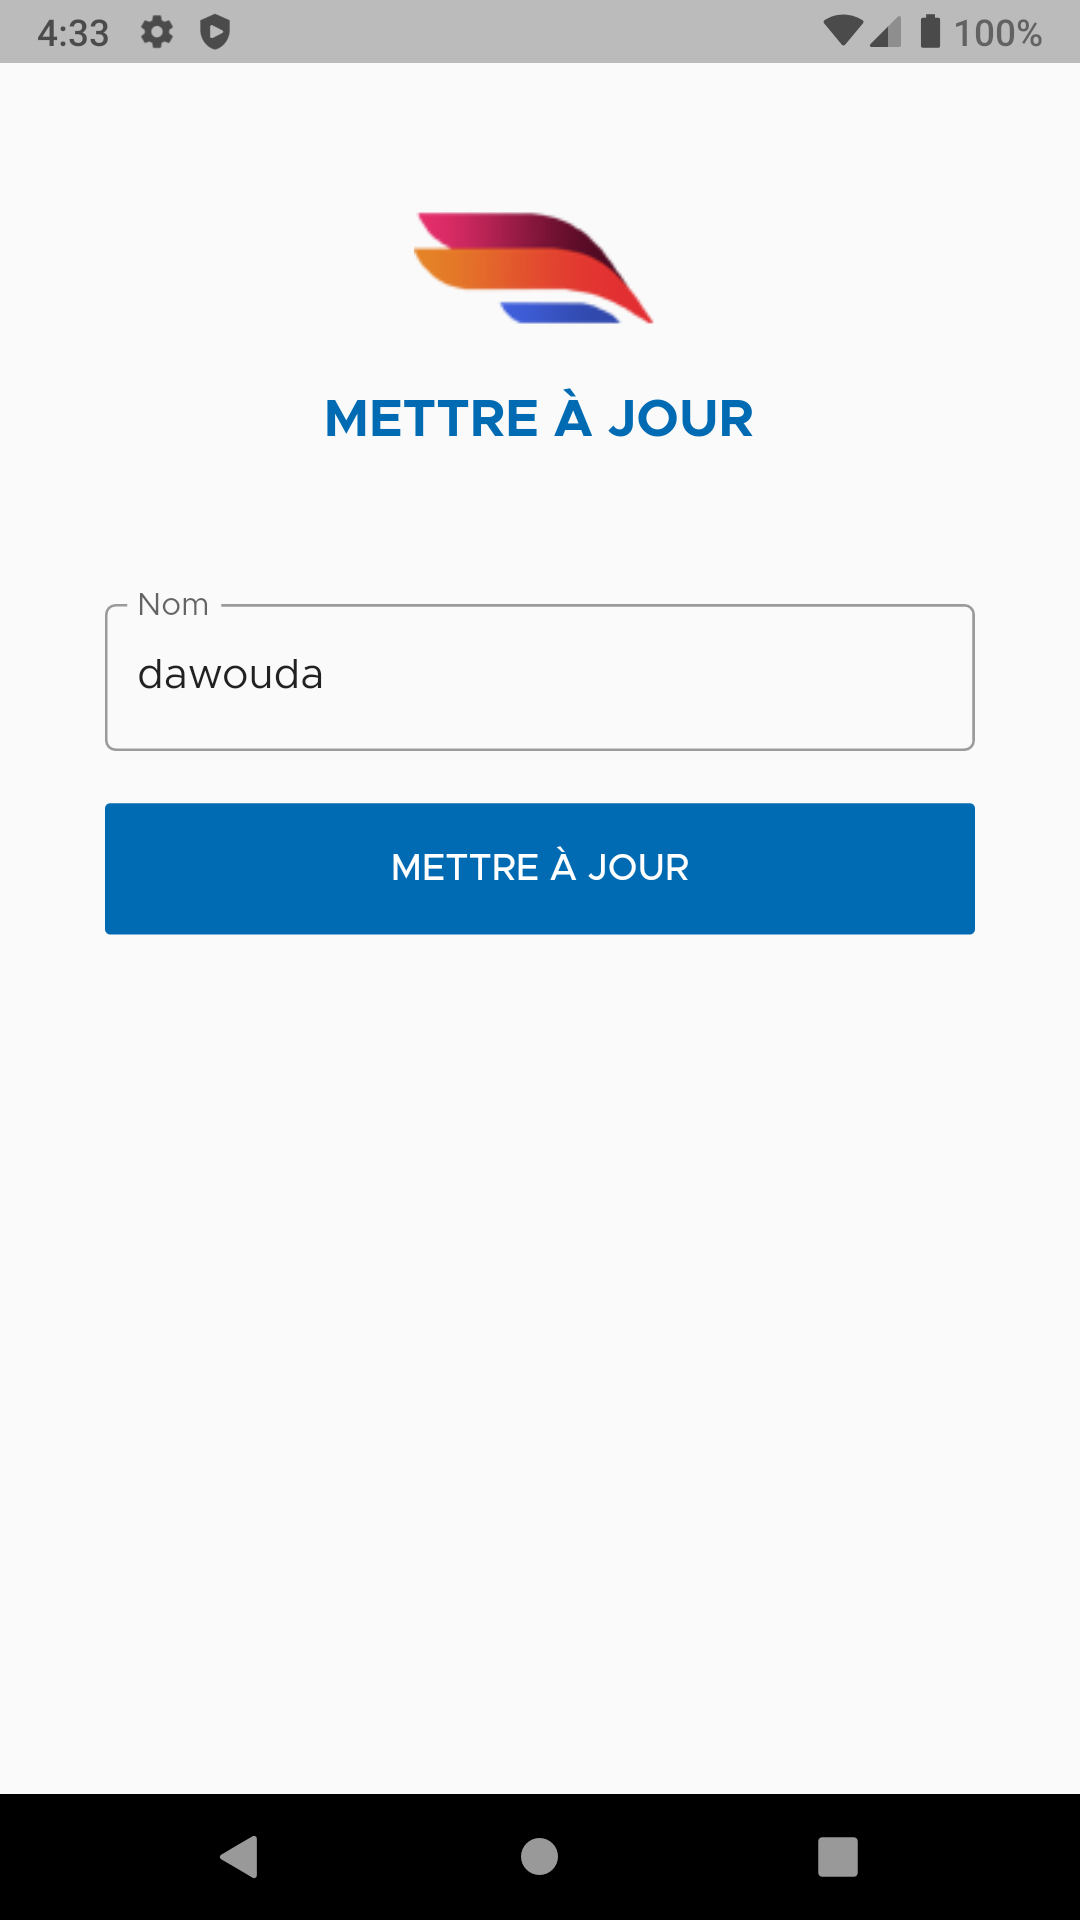
\includegraphics[width=\textwidth]{./Template LaTeX/Images/From_emu/A_up_s.png}
		\caption{Mettre à jour un compte}
		\label{fig:five over x}
	\end{subfigure}
	\newline
	\centering
	\begin{subfigure}{0.3\textwidth}
		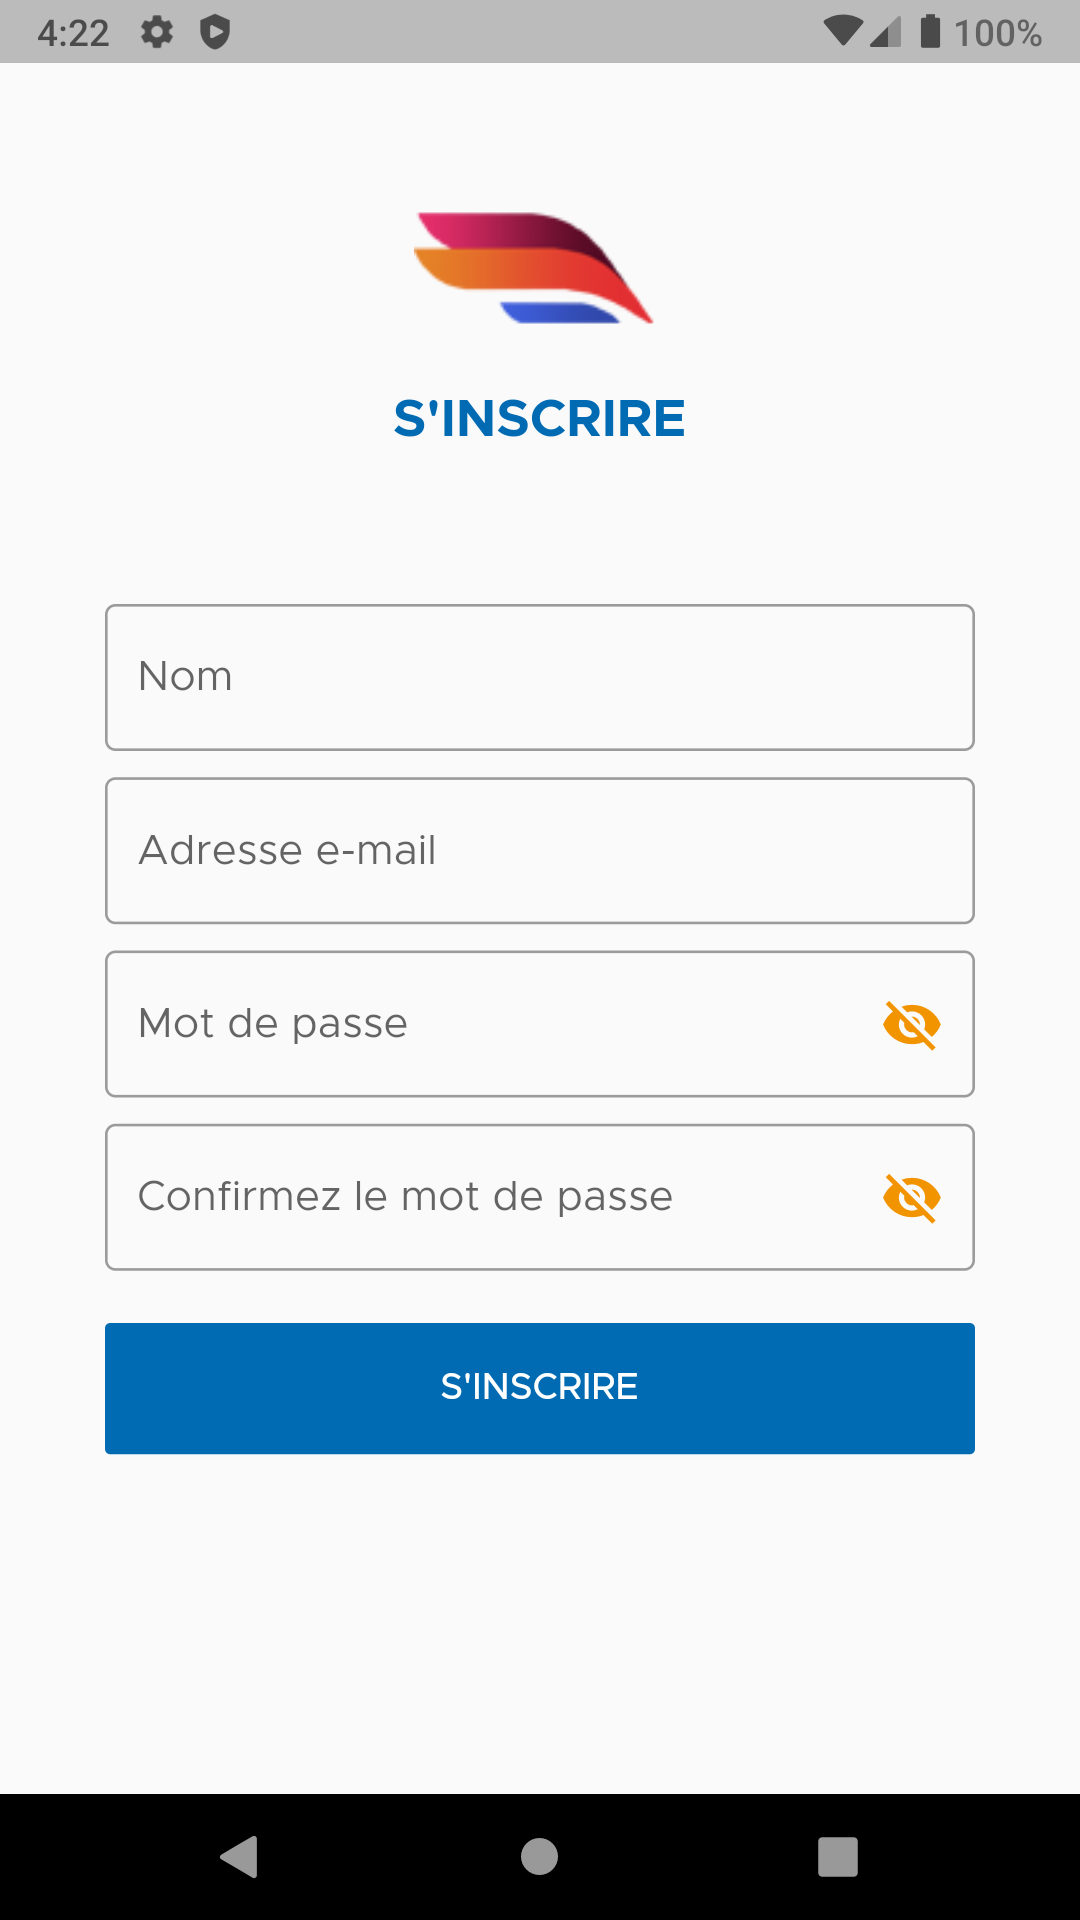
\includegraphics[width=\hsize, valign=m ]{./Template LaTeX/Images/From_emu/A_add_s.png}
		\caption{Ajouter un compte}
		\label{fig.SICAPI}
	\end{subfigure}
	%\qquad\tikz[baseline=-\baselineskip]\draw[ultra thick,->] (0,0) -- ++ (1,0);\qquad
	
	\caption{Interface du compte administrateur
	}
	\label{Home}
\end{figure}
%%%%%%%%%%%%%%%%%%%%%%%%%%%%%%%%%%%%%%%%%%%%%%%%%%%%%%%%%%%%%
\newpage
\item \textbf{L’interface du compte service client
	:} 
La figure~\ref{serviceCl} représente la page principale de l’application pour le compte service client C’est à partir de cette fenêtre l'utilisateur peut répondre aux clients.
\begin{figure}
	\centering
	\begin{subfigure}{0.3\textwidth}
		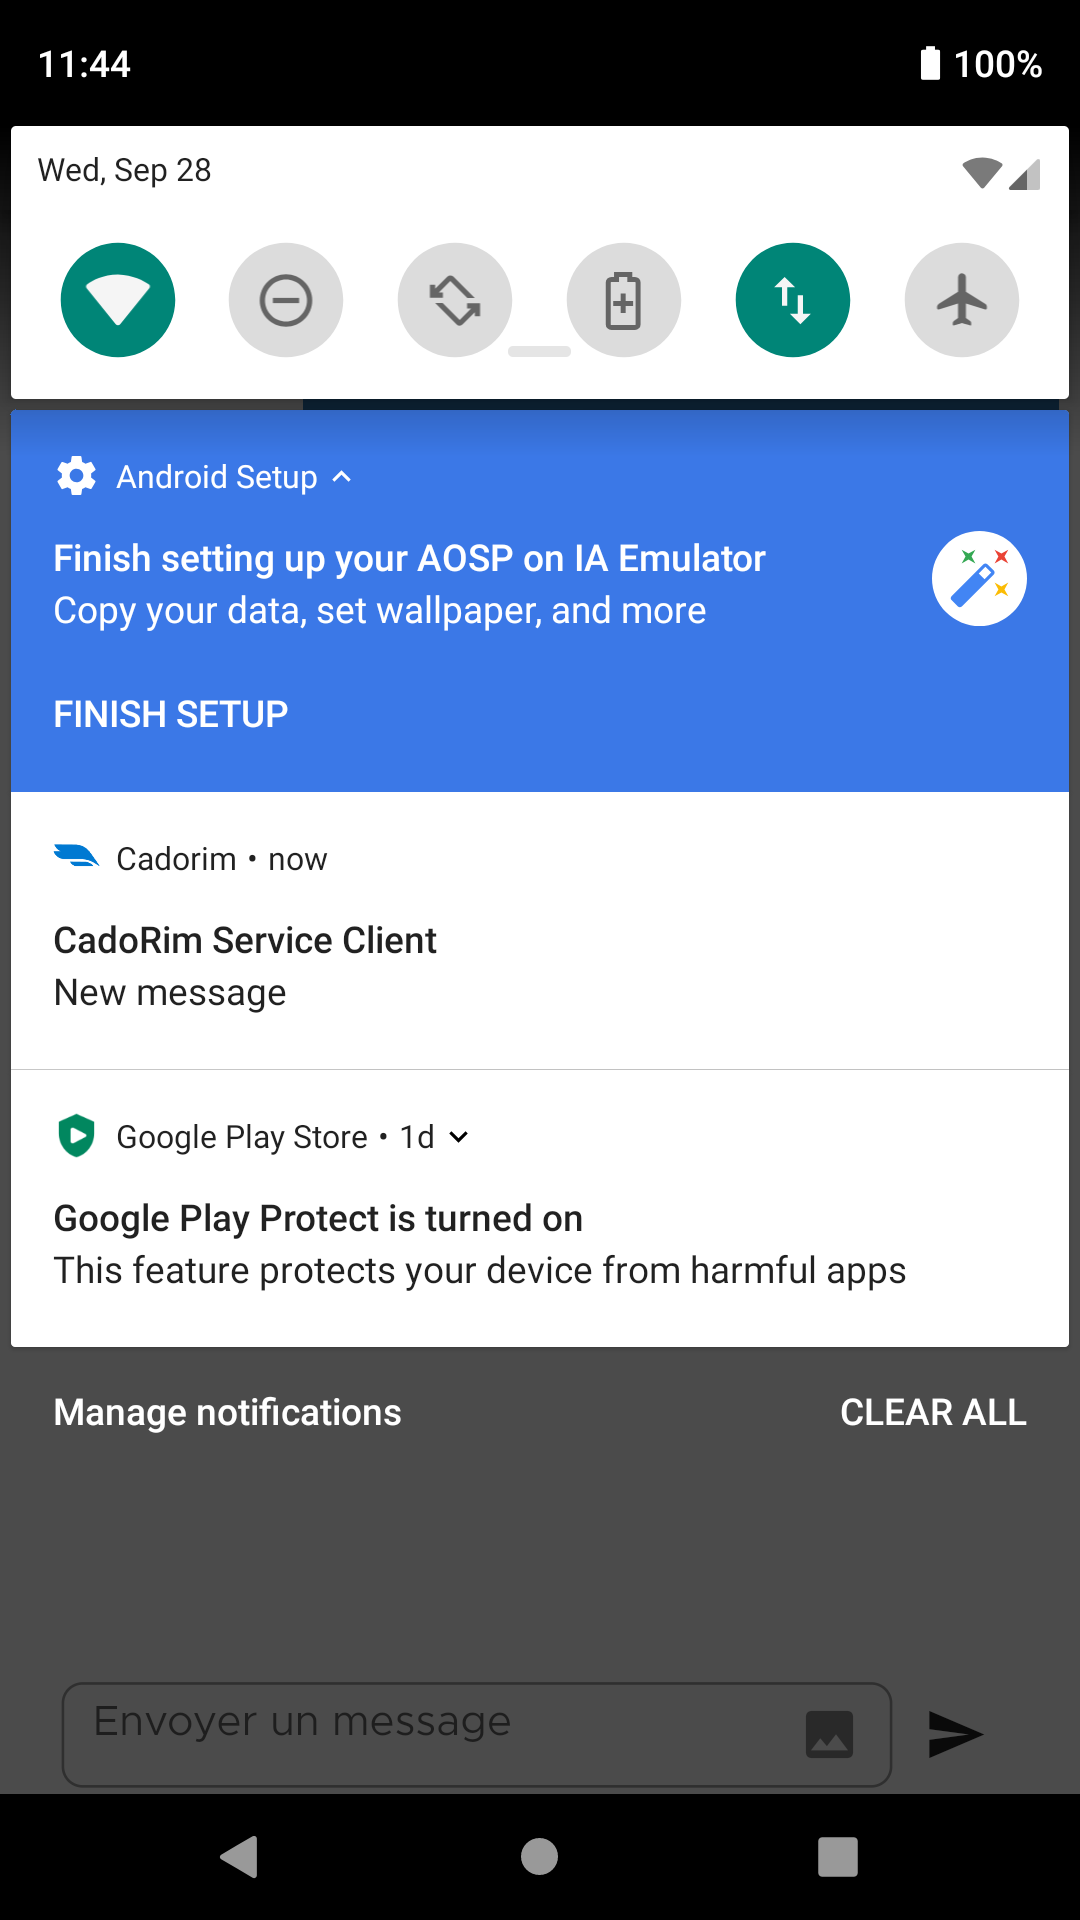
\includegraphics[width=\hsize, valign=m ]{./Template LaTeX/Images/From_emu/a.png}
		\caption{Notification}
		\label{klk}
	\end{subfigure}
	\begin{subfigure}{0.3\textwidth}
		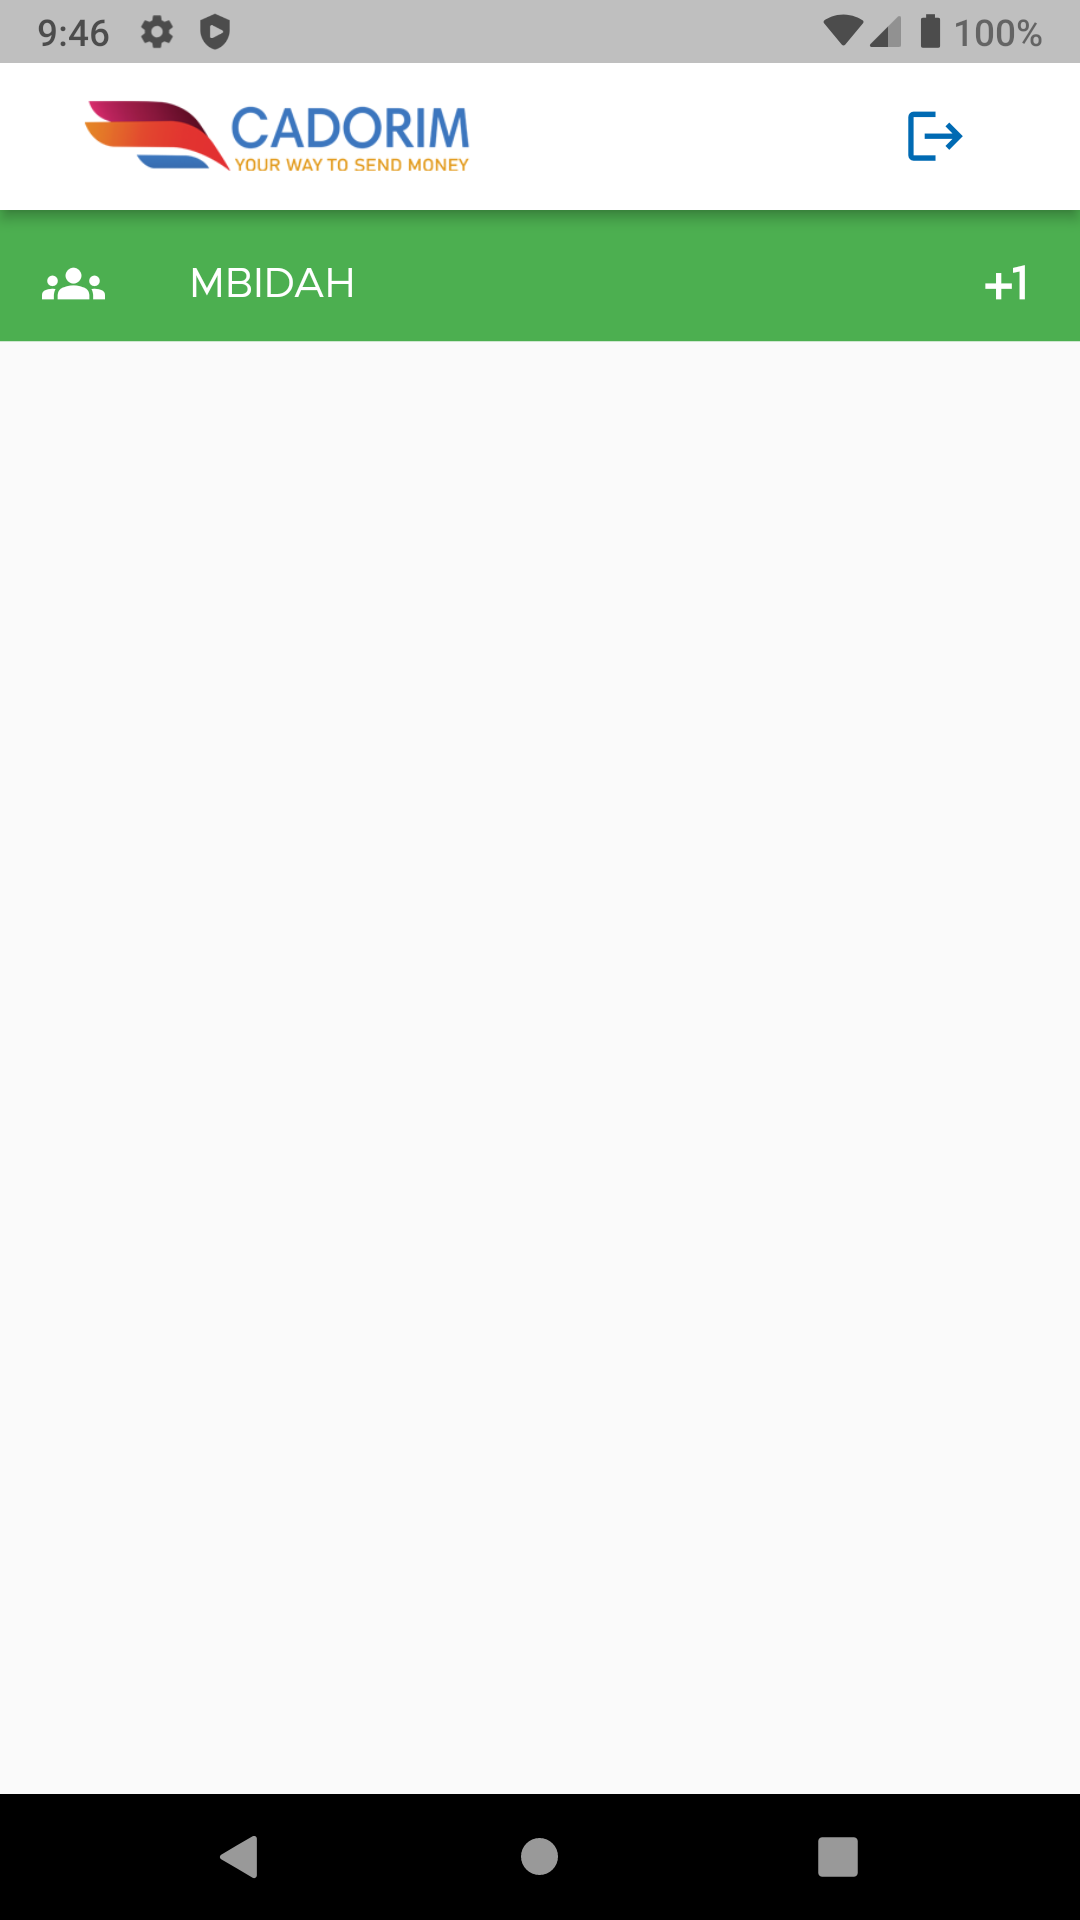
\includegraphics[width=\hsize, valign=m ]{./Template LaTeX/Images/From_emu/no_vue.png}
		\caption{Interface d’accueil}
		\label{klk}
	\end{subfigure}
	\begin{subfigure}{0.3\textwidth}
		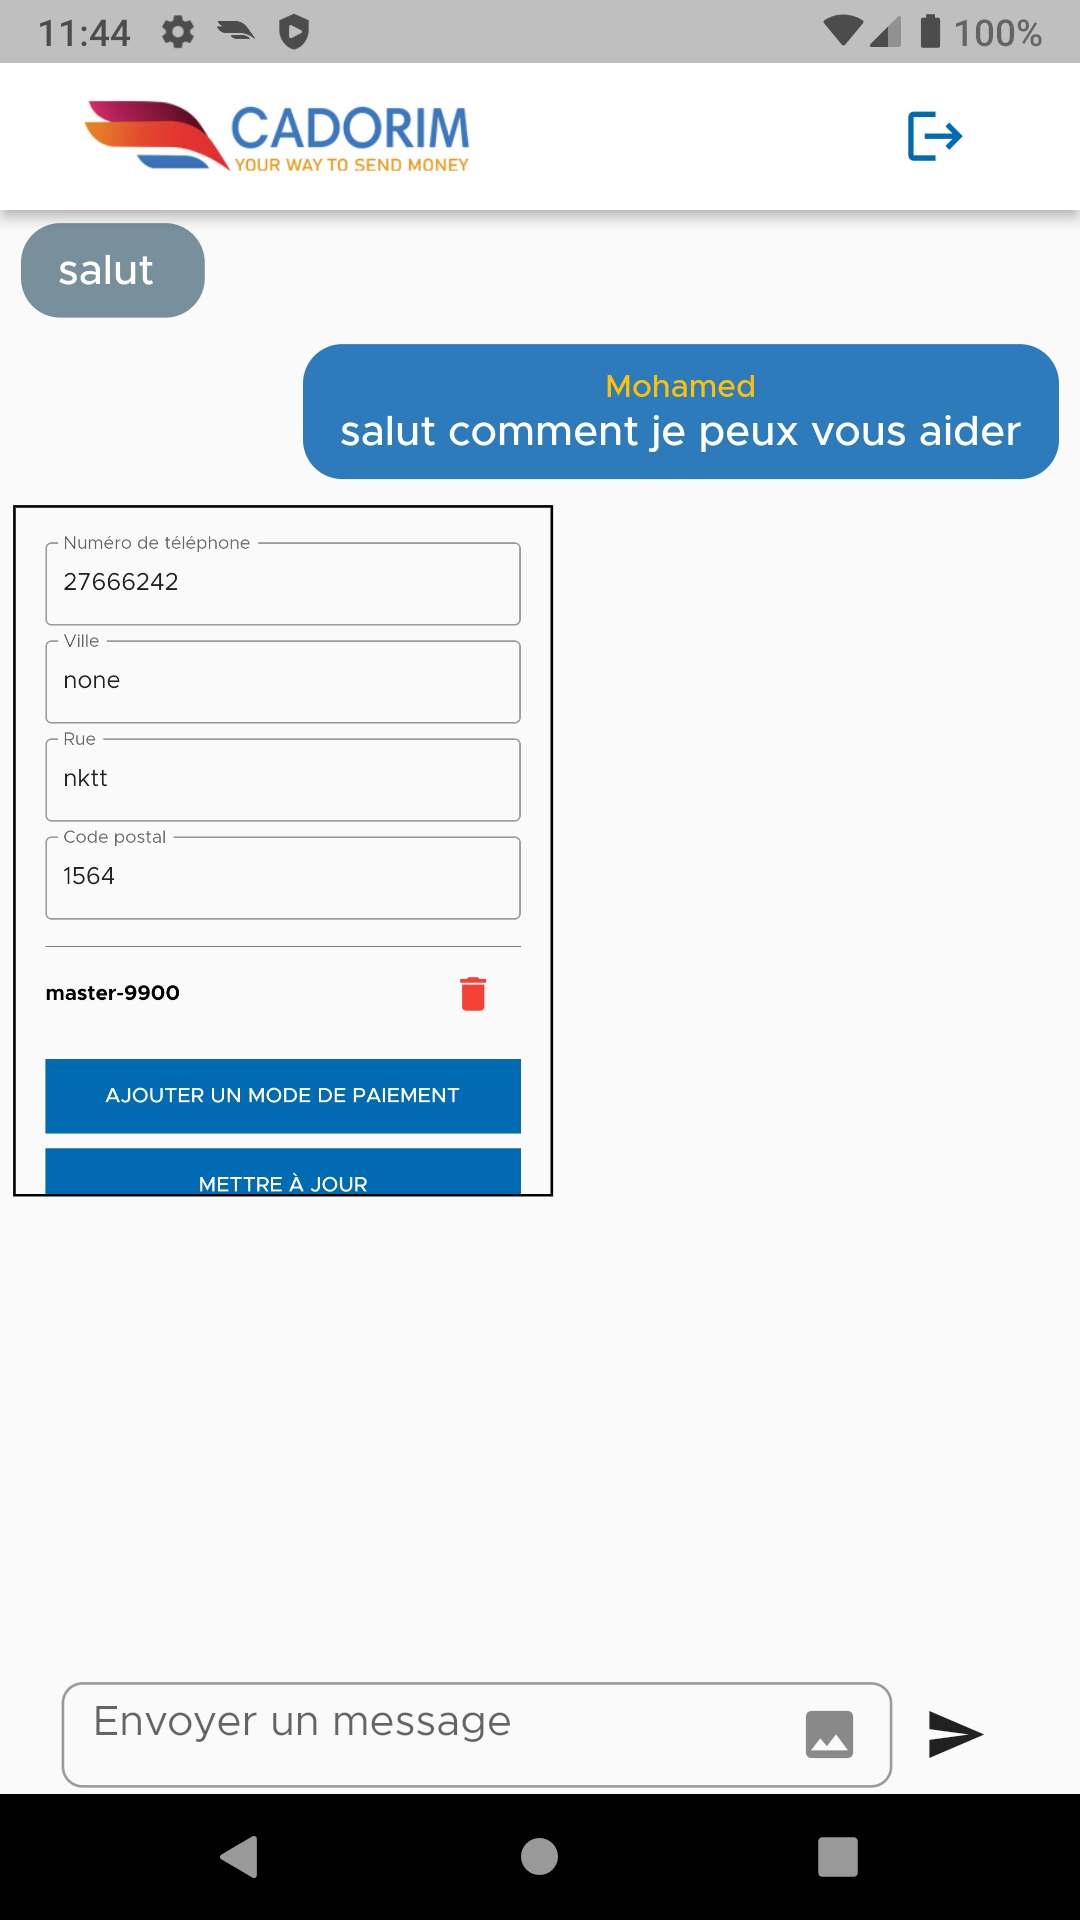
\includegraphics[width=\hsize, valign=m ]{./Template LaTeX/Images/From_emu/b.png}
		\caption{Interface de discussion}
		\label{klk}
	\end{subfigure}
	\caption{Interface du compte service client
	}
	\label{serviceCl}
\end{figure}
\end{itemize}


